\chapter{Evaluation}
\label{chap:evaluation}

\section{Overview}
\label{sec:evaluation-overview}

As we have seen so far, several parameters are used in our implementation. For instance, one can enable or disable the preprocessing step that removes the unique sequences, or do the same for the summariser. Moreover, we have implemented two different clustering algorithms that may lead to different results, in terms of the sequences that are clustered together. This prompts us to evaluate different versions of the system which, however, should vary as little as possible with respect to the different conditions. Ideally, when evaluating between different versions of a system, these versions may only differ by a single parameter, in order to draw appropriate conclusions.

In the next section we are going to explain our decision to evaluate the system's results using the examples written by the developers of the libraries, rather than writing our own gold standard examples.

After that, we present the different versions that aim to be used for the evaluation of the system, as well as the dataset used. Then, we divide the evaluation process into several experiments where, for each one, we clearly point out the hypothesis that is going to be tested. This step-by-step evaluation process will enable us to evaluate different aspects of the system and of the results. Additionally, the last experiment intends to evaluate the key hypothesis of the current dissertation.

We decided to use only the \texttt{Twitter4J} dataset in the conducted experiments, as we noted that, even when using this single dataset, we draw numerous interesting conclusions. Moreover, the hypotheses defined in the experiments may be well evaluated using this dataset.

To avoid any confusion, we firstly describe three main terms that are going to be used in the evaluation process.

\begin{description}
\item[Sequence] A sequence refers to an API call sequence. When this term is used in the evaluation metrics, this indicates the API call sequences of the snippets mined by our system.
\item[Snippet] A snippet refers to a Java code fragment mined by our system. The mined snippets are the results of our system.
\item[Example] An example refers to a handwritten Java code fragment, which is part of the \texttt{examples} directory of the target API. 
\end{description}


\section{Evaluating Using the \texttt{examples} Directory}
\label{sec:examples-evaluation}

In the majority of the publications in the field of API usage mining, the authors evaluate their systems with the aid of user studies. However, as we mentioned in \Cref{chap:introduction}, this inevitably leads to subjective results. Furthermore, \nolink{\citeauthor{Young:2005}} \cite{Young:2005} correctly point out that ``the human eye is a slow, expensive, and unreliable instrument for judging test outcomes''. This prompts us to use a more automatic way of evaluating our system. Taking into account that writing our own gold standard examples would also lead to subjective results, while it is moreover time consuming, a better approach would be to look for such gold standard examples in the internet. Fortunately, the developers of several APIs include such examples in their repositories. We believe that this is a really valuable information that could be usefully utilised for the evaluation of systems that perform API usage mining. In addition to that, the evaluation using handwritten examples that exist in the \texttt{examples} directory of the target libraries, has already been tested in \cite{Fowkes2:2015}, where the system under evaluation mines API call sequences. Therefore, we decided to use a similar methodology, with the intention of evaluating snippets rather than sequences. To the best of our knowledge, this is the first system to be evaluated using this methodology, and we hope that the outcome would be interesting enough, in the hope that this methodology will be used for the evaluation of similar systems in the future. After all, many popular authors in the field of IR insinuate that this field seems to lack of efficient and objective evaluation techniques \cite{Manning:2008}, and our approach may be helpful on that.


\section{Versions of the System Under Evaluation}
\label{sec:evaluation-versions}

\Cref{tables:evaluation-versions} illustrates the different versions of our system that are going to be considered during the evaluation process.

\begin{table}[ht]
\centering
\small
\caption[System versions]{Different versions of the system that are going to be considered under the evaluation process.}
\label{tables:evaluation-versions}
\begin{tabular}{lllll}
\toprule
\multirow{2}{*}[3pt]{Version} & Unique Sequences & Clustering & \multirow{2}{*}[3pt]{Summariser} \\[-5pt]
& Removal & Algorithm & \\
\midrule
$RemUniqNaivNoSum$ & ON & Naive & OFF \\
$RemUniqNaivSum$ & ON & Naive & ON \\
$KeepUniqNaivSum$ & OFF & Naive & ON \\
$KeepUniqKMedoidsSum$ & OFF & $k$-medoids & ON \\
$KeepUniqHDBSCANSum$ & OFF & HDBSCAN & ON \\
\bottomrule
\end{tabular}
\end{table}

As might be seen, the first parameter is related to the preprocessing step, and indicates whether the unique sequences are going to be removed or not. The second parameter is the clustering algorithm to be used, with the aim of clustering the API call sequences. The \textit{naive} algorithm has not been analysed in \Cref{chap:implementation}, as it purely clusters identical sequences together. In fact, there was no need to implement a different algorithm, as this could be seen as a $k$-medoids version, where the number of clusters equals the number of the non-identical sequences after the preprocessing step. The versions that use this algorithm are going to reveal whether a more powerful technique, that clusters similar rather than identical sequences, leads to better results. Finally, the summariser that leverages the implemented summarisation algorithm can be enabled or disabled in advance.

The values of the input parameters for the $k$-medoids and the HDBSCAN clustering algorithms are going to be presented in the experiments.


\section{Dataset}
\label{sec:evaluation-dataset}

As regards the dataset used, we make use of the \texttt{Twitter4J} dataset, which is part of the \textsc{Example} dataset, used in \cite{Fowkes2:2015}. This dataset targets the \texttt{Twitter4J} API, and summary statistics for the client code, as well as for the \texttt{examples} that are related to this dataset are presented in \Cref{tables:dataset-summary}. Taking into account that we are going to evaluate the results of the system using the handwritten examples in the \texttt{examples} directory as our gold standards, we decided not to split the dataset into a training and a test set. That is, the training set is the entire client code, while the test set includes the source code in the \texttt{examples} directory.

\begin{table}[ht]
\centering
\small
\caption[Dataset summary]{Summary of the \texttt{Twitter4J} dataset, which is part of the \textsc{Examples} dataset presented in \cite{Fowkes2:2015}.}
\label{tables:dataset-summary}
\begin{tabular}{lr}
\toprule
Attribute & Value \\
\midrule
No. client files & 549 \\
Client LOCs & 96,010 \\
No. API classes in client files & 81 \\
No. API methods in client files & 475 \\
No. transactions in the \texttt{.arff} file & 1,066 \\
No. singleton sequences in the \texttt{.arff} file & 367 \\
No. pseudo-singleton sequences in the \texttt{.arff} file & 39 \\
No. unique sequences in the \texttt{.arff} file & 585 \\
No. example files & 89 \\
Example LOCs & 5,458 \\
\bottomrule
\end{tabular}
\end{table}


\section{Evaluation Metrics}
\label{sec:evaluation-metrics}

In this section we present the metrics used in an attempt to evaluate the system. We make use of popular metrics related to the precision of the system, as well as to the coverage of the API methods in the dataset. Moreover, we define a metric that would enable us to evaluate whether presenting snippets rather than sequences is of more value to the developers. Furthermore, we make use of two quantitative metrics used in \cite{Buse:2012}, with the purpose of evaluating the summarisation algorithm. We point out that the expression $|x|$ is a shortcut for the expression ``number of $x$''.


\subsection{Precision Metrics}
\label{subsec:evaluation-precision}

Regarding the overall precision of the system, we define the $sequence\_precision$ and the $snippet\_precision$, in \Cref{eq:sequence-precision,eq:snippet-precision}, respectively.
%
\vspace{1ex}
\begin{equation}
 \label{eq:sequence-precision}
 \centering
  sequence\_precision = 
  \frac{ | \text{sequences contained in at least one example} | }
       { | \text{sequences} | }
\end{equation}
%
\begin{equation}
 \label{eq:snippet-precision}
 \centering
  snippet\_precision = 
  \frac{ \displaystyle\sum_{i=1}^{|snippets|}
   \frac{ | tokens\_snippet_i\, \cap \, tokens\_gold_{snippet_i} | }
  		{ | tokens\_snippet_i | } }
        { | \text{snippets} | }
 \vspace{2ex}
\end{equation}
%
where $tokens\_gold_{snippet_i}$ are the tokens in the example that best matches to $snippet_i$.

The $sequence\_precision$ metric is computed based on the API call sequences between a mined snippet and a handwritten example, while the $snippet\_precision$ takes into account the entire snippets. More specifically, the latter metric computes the overlap between a snippet and its most similar example, in terms of Java tokens. The process followed in order to extract the tokens and to compute the $snippet\_precision$ metric, is extensively analysed in \Cref{sec:snippet-based-metrics}.

We also define the $matched\_snippet\_precision$, in \Cref{eq:matched-snippet-precision}, with the intention of eliminating the effect of the snippets that have not been matched to any of the examples, to the value of the $snippet\_precision$ metric.
\vspace{1.5ex}
%
\begin{equation}
 \label{eq:matched-snippet-precision}
 \centering
  matched\_snippet\_precision = 
  \frac{ \displaystyle\sum_{i=1}^{m} 
  	\frac{ | tokens\_snippet_i \, \cap \, tokens\_gold_{snippet_i} | }
  		 { | tokens\_snippet_i | } }
       { m }
 \vspace{1.5ex}
\end{equation}
%
where $m$ is the number of snippets that match to at least one example.


\subsubsection{Evaluating the Precision of Ranked Results}
\label{subsubsec:evaluation-ranked}

Taking into account that our system returns a ranked list of snippets, we also make use of the \textit{precision at top $k$} ($precision@k$), which is also known as \textit{precision at cut-off $k$}. This metric indicates the precision calculated for the set of the top $k$ documents returned, and is heavily used for the evaluation of ranked documents\footnote{\url{http://nlp.stanford.edu/IR-book/html/htmledition/evaluation-of-ranked-retrieval-results-1.html}}. Such a metric would enable us to plot the precision for different values of $k$, while it would facilitate the comparison between versions of the system that return a different number of snippets. Based on this, and similarly to the precision metrics presented above, we firstly define the average sequence precision at top $k$ ($avg\_seq\_prec@k$), in \Cref{eq:avg-sequence-precision-atk}\footnote{Usually, there is a confusion on how the average at top $k$ is computed. In this evaluation, we use the formula in a similar way to that presented in \url{https://www.kaggle.com/c/avito-prohibited-content/forums/t/9584/average-precision-at-k-ap-k/50976\#post50976}}.
\vspace{1ex}
%
\begin{equation}
 \label{eq:avg-sequence-precision-atk}
 \centering
  avg\_seq\_prec@k = 
  \frac{ \displaystyle\sum_{i=1}^{k}
    seq\_prec@i }
       { k }
\end{equation}
%
where:
\vspace{1.5ex}
%
\begin{equation*}
 \label{eq:sequence-precision-ati}
 \centering
  seq\_prec@i = 
  \frac{ | \text{matched sequences at top $i$} | }
       { i }
 \vspace{1.5ex}
\end{equation*}
%
In a similar manner, the average snippet precision at top $k$ ($avg\_snip\_prec@k$) is defined in \Cref{eq:avg-snippet-precision-atk}.
\vspace{1.5ex}
%
\begin{equation}
 \label{eq:avg-snippet-precision-atk}
 \centering
  avg\_snip\_prec@k = 
  \frac{ \displaystyle\sum_{i=1}^{k}
    snip\_prec@i }
       { k }
 \vspace{1.5ex}
\end{equation}
%
where:
%
\vspace{1.5ex}
\begin{equation*}
 \label{eq:snippet-precision-ati}
 \centering
  snip\_prec@i = 
  \frac{ \displaystyle\sum_{j=1}^{i}
   \frac{ | tokens\_snippet_j\, \cap \, tokens\_gold_{snippet_j} | }
  		{ | tokens\_snippet_j | } }
        { i }
 \vspace{1.5ex}
\end{equation*}
%
Another metric used in order to evaluate the quality of the sequences, as well as of the snippets, is the \textit{Normalised Discounted Cumulative Gain\footnote{\url{https://www.kaggle.com/wiki/NormalizedDiscountedCumulativeGain}}}, which uses the graded relevance as a measure of usefulness. 

The formula of this metric is shown in \Cref{eq:ndcg}.
\vspace{1ex}
%
\begin{equation}
 \label{eq:ndcg}
 \centering
  nDCG_k = 
  \frac{ DCG_k } { IDCG_k }
\end{equation}
%
where:
\vspace{1ex}
%
\begin{equation*}
 \centering
  DCG_k = \displaystyle\sum_{i=1}^k
  \frac{  2^{rel_i}-1 } 
       { \log_2 (i+1) }
  \vspace{1.5ex}
\end{equation*}
%
\normalsize
and $IDCG_k$ is the maximum possible (ideal) $DCG$. Note that the value of $rel_i$ indicates the relevance of the $i_{th}$ recommended entity to the query.

Based on the above, we define the $sequence\_nDCG_k$ and the $snippet\_nDCG_k$. Regarding the value of $rel_i$, when computing the $sequence\_nDCG_k$, this is set to $1.0$ if the snippet's sequence is contained in at least one example, and to $0.0$ otherwise. This reveals that we consider it as a boolean variable. On the other hand, for the $snippet\_nDCG_k$, the value of $rel_i$ indicates the similarity of a snippet to the example it best matches to, and lies in the range [$0.0$,$1.0$]. The $IDCG_k$ is in both cases set to $1.0$.


\subsection{Metrics Used for the Evaluation of the Key Hypothesis}
\label{subsec:evaluation-key-hypothesis}

With the purpose of evaluating the key hypothesis of the current dissertation, which is that presenting snippets rather than sequences would be of greater value to the developers, we additionally define the $addit\_snippet\_info$ metric, in \Cref{eq:addit-info}. This metric indicates the amount of information that is revealed when presenting snippets instead of sequences. In other words, it shows how much information is suppressed when presenting sequences instead of snippets. In order to compute this information, we can see an API call sequence as a sequence of tokens, where a token is the name of an API method, and refer to them as the \textit{sequence-tokens} of a mined snippet. Then, the Java tokens extracted using the process in \Cref{sec:snippet-based-metrics} are referred to as the \textit{snippet-tokens} of the mined snippet.
\vspace{1ex}
%
\begin{equation}
 \label{eq:addit-info}
 \centering
  addit\_snippet\_info = 
  \frac{ \displaystyle\sum_{i=1}^{m} 
  	\frac{ | tokens\_snippet_i \, \cap \, tokens\_gold_{snippet_i} |}
  		 { | tokens\_sequence_{snippet_i} \, \cap \, tokens\_gold_{snippet_i} | } }
       { m }
 \vspace{0.5ex}
\end{equation}
%
where $tokens\_sequence_{snippet_i}$ are the tokens of the sequence associated with $snippet_i$ (\textit{sequence-tokens}), and $m$ is the number of snippets that match to at least one example.


\subsection{Coverage Metrics}
\label{subsec:evaluation-coverage}

On top of the aforementioned metrics, we also compute the percentage of the API methods covered by the mined snippets. This is a popular evaluation metric in the field of API usage mining, which is also considered in one of the few recent publications that aim to build API usage example metrics \cite{Radevski:2016}. This metric is going to facilitate the decision on the best version of the system, as we will be able to investigate whether there is a trade-off between the precision of the mined snippets and the coverage of the API, in terms of the API's methods. Its formula is shown in \Cref{eq:coverage}.
\vspace{1.5ex}
%
\begin{equation}
 \label{eq:coverage}
 \centering
  coverage\_of\_API\_methods =  
  \frac{ | \text{API methods covered by the mined snippets} | }
       { | \text{API methods in the dataset} | }
 \vspace{1.5ex}
\end{equation}
%
Note that the coverage is computed over the API methods in the dataset (\texttt{.arff} file), rather than over the total number of the methods defined in the API. This decision is based on the fact that, in case an API method does not exist in any of the files in our local repository, there is no way to cover this method. In this way, we focus on the approach followed to solve the problem, rather than on whether the dataset used covers the API.


\subsection{Size and Readability Metrics}
\label{subsec:evaluation-size-readability}

In order to evaluate the summarisation algorithm, we make use of two quantitative metrics, which have been used for the evaluation of similar systems \cite{Buse:2012}; the \textit{Physical Lines of Code} (PLOCs) and the \textit{readability} metric, which are analysed below.

In order to count the PLOCs of a source code file, we use the \textit{loc-counter} tool\footnote{\url{https://java.net/projects/loc-counter/pages/Home}}, which counts any line that has more than three non-blank characters. It is clear that this is not a normalised metric (e.g. in the range [$0.0$, $1.0$]).

As regards the readability of a source code file, we use the appropriate tool from \nolink{\citeauthor{Buse:2008}}\footnote{\url{http://www.arrestedcomputing.com/readability}}, which is based on the authors' work in \cite{Buse:2008}. This metric is based on human studies and has been proven efficient enough to agree with a large set of human annotators. Given a Java source code file, the tool outputs a value in the range [$0.0$, $1.0$], where a higher value indicates a more readable snippet.

Based on the above, we define the $avg\_snippet\_readability$ in \Cref{eq:readability}, as well as the $avg\_snippet\_PLOCs$ in \Cref{eq:plocs}.
\vspace{1.5ex}
%
\begin{equation}
 \label{eq:readability}
 \centering
  avg\_snippet\_readability = 
  \frac{ \displaystyle\sum_{i=1}^{|snippets|}\text{readability of $snippet_i$} }
       { | \text{snippets} | }
\end{equation}
\vspace{-1ex}
%
\begin{equation}
 \label{eq:plocs}
 \centering
  avg\_snippet\_PLOCs = 
  \frac{ \displaystyle\sum_{i=1}^{|snippets|}\text{PLOCs of $snippet_i$} }
       { | \text{snippets} | }
  \vspace{1.5ex}
\end{equation}
%
Having defined and explained the evaluation metrics, we can now go on with the experiments that have been conducted in order to evaluate the system.


\section{Experiment 1 - Evaluating the Summarisation Algorithm}
\label{sec:evaluation-exp1}

In the experiment of this section, we are going to investigate whether the integration of the implemented summarisation algorithm improves the results of the system. For this purpose, we use the first two versions presented in \Cref{tables:evaluation-versions}, namely the $RemUniqNaivSum$ and the $RemUniqNaivNoSum$ versions. In both of them the unique sequences are removed before the clustering process, while they both use the \textit{naive} clustering technique, where only identical sequences are clustered together. The hypothesis under evaluation is described below:

\begin{hypothesis}
The summarisation algorithm leads to more concise and readable snippets, while improving their precision with respect to the handwritten examples.
\end{hypothesis}


\subsection{Quantitative results}
\label{subsec:evaluation-exp1-quantitative}

\Cref{tables:evaluation-summariser} shows the values of the metrics used for the evaluation of the summariser. It is clear that the precision of the system, with respect to the handwritten examples, has been improved. This is mostly revealed by the spectacular increase in the $matched\_snippet\_precision$ metric, where only the matched snippets affect the metric's value. Interpreting this value, well above than $2/3$ of the content of any mined snippet is used by its associated handwritten example, when using the summarisation algorithm.

\begin{table}[ht]
\centering
\small
\caption[Evaluation metrics\protect\\($RemUniqNaivNoSum$, $RemUniqNaivSum$)]{Evaluation metrics for the version that does not make use of the summariser ($RemUniqNaivNoSum$), and for this that does leverage it ($RemUniqNaivSum$).}
\label{tables:evaluation-summariser}
\begin{tabular}{lll}
\toprule
Metric & $RemUniqNaivNoSum$ & $RemUniqNaivSum$ \\
\midrule
$snippet\_precision$ & 0.14 & 0.19 \\
$matched\_snippet\_precision$ & 0.49 & 0.69 \\
$avg\_snippet\_readability$ & 0.17 & 0.37 \\
$avg\_snippet\_PLOCs$ & 13.13 & 8.09 \\
\bottomrule
\end{tabular}
\end{table}

Regarding the readability of the snippets, this is more than doubled when leveraging the summariser. We should point out here that, although the readability may seem low, even when using the summariser, this is mainly due to the fact that the readability metric considers features such as the lines' length or even the identifiers' length, as discussed in its designers' paper \cite{Buse:2008}.

In addition to the readability of the snippets, there is a decrease in the number of PLOCs. This is definitely a result of the non-API statements removal, especially if we take into account that the summariser also resolves any variable types; a fact that should lead to longer snippets rather than to shorter ones. This decrease in the PLOCs would be more clear if we exclude the additional statements that aim to resolve variable types. In that case, we find out that the value of the $avg\_snippet\_PLOCs$ is further decreased to almost 5 PLOCs. Recalling the notion of the \textit{concise code}, as this has been defined in \cite{Nasehi:2012}, and mentioned in \Cref{sec:source-code-summarisation}, we could claim that the summarisation algorithm successfully leads to concise snippets.


\subsection{Visualising the Results}
\label{subsec:evaluation-exp1-plots}

In order to better interpret the results, we firstly plot the sequence precision at top $k$, and the $snippet\_nDCG_k$, in \Cref{res:exp1-precision,res:exp1-ndcg}, respectively.

It is clear from \Cref{res:exp1-precision} that the version that uses the summariser mines more precise snippets than the one that does not use it, for any value of $k$. The difference between the two versions is furthermore illustrated in \Cref{res:exp1-ndcg}, where the relevance is graded, with respect to the ranking. Both plots indicate a downward trend in the precision metric, which is justified by the fact that the mined snippets that are placed in lower positions are more complex; they normally contain a large number of API calls.

\begin{figure}
\ffigbox
{%
  \begin{subfloatrow}[2]
  \ffigbox[\FBwidth]
    {\caption{}\label{res:exp1-precision}}
    {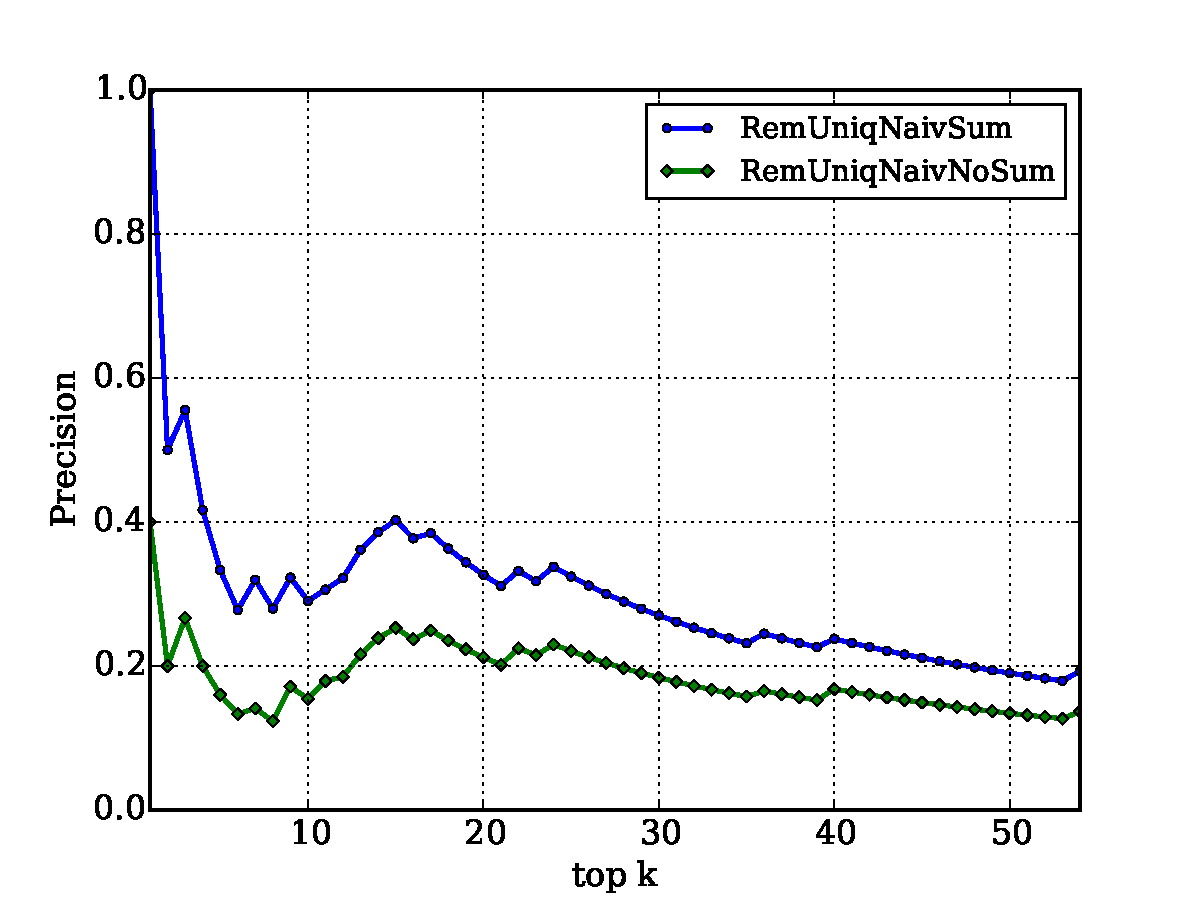
\includegraphics[width=0.45\textwidth]{results/exp1-precision.pdf}}
  \hspace{1em}%
  \ffigbox[\FBwidth]
    {\caption{}\label{res:exp1-ndcg}}
    {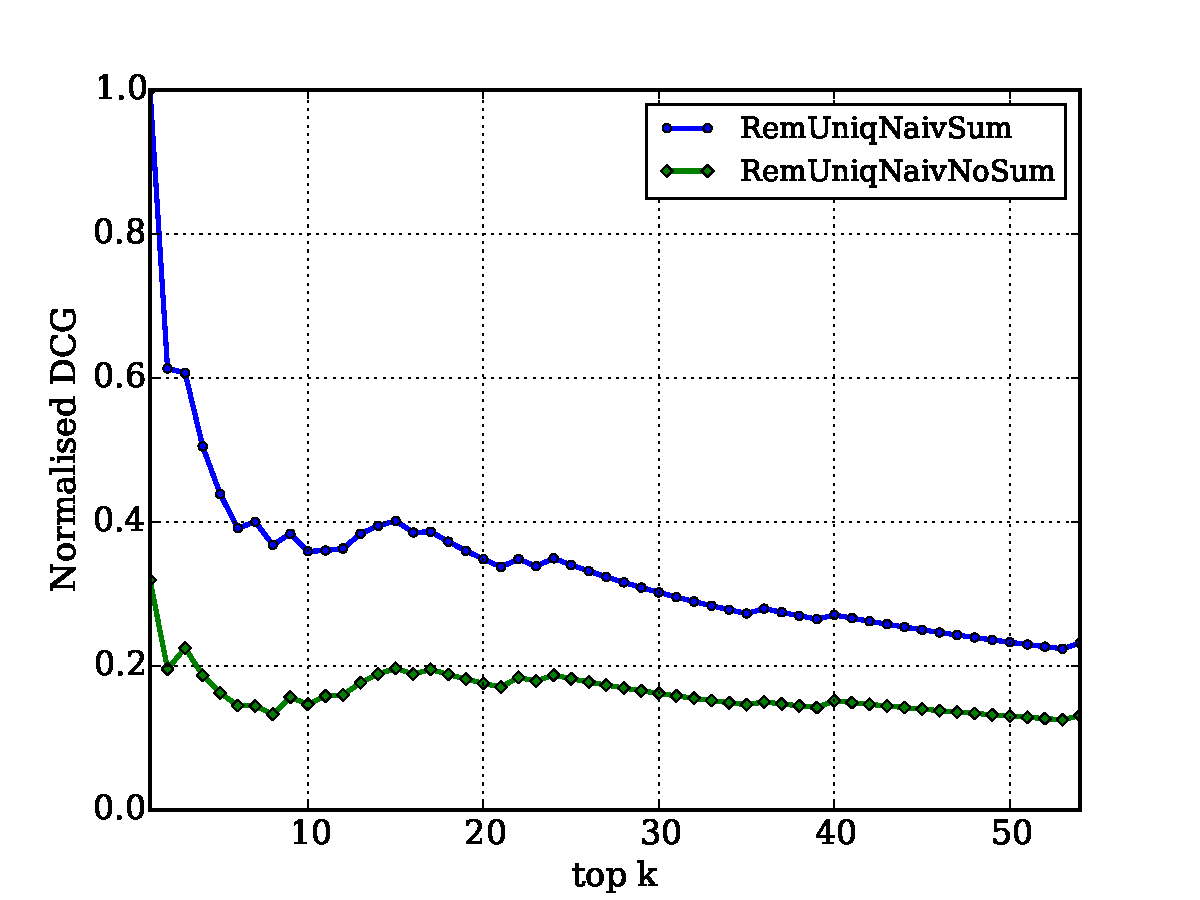
\includegraphics[width=0.45\textwidth]{results/exp1-ndcg.pdf}}
  \end{subfloatrow}}
  {\caption[Illustration of the precision metrics\protect\\($RemUniqNaivNoSum$,$RemUniqNaivNoSum$)]{Figures illustrating (\subref{res:exp1-precision}) the $snippet\_precision@k$, and (\subref{res:exp1-ndcg}) the $snippet\_nDCG_k$ for both versions.}
\label{res:exp1-prec-ndcg}}
\end{figure}

We also plot the distribution of the mined snippets in terms of their readability, in \Cref{res:exp1-readability}, as well as in terms of their PLOCs, in \Cref{res:exp1-plocs}. As depicted in \Cref{res:exp1-readability}, the version that leverages the summariser generates almost $10$ snippets with readability $\geq 0.8$, out of the $54$ that are mined in total, while the version that does not make use of the summarisation algorithm does not mine any snippet with a readability in that range. Moreover, almost half of the snippets generated by the $RemUniqNaivSum$ version have a readability $\geq 0.5$. Inspecting the readability of each snippet manually, showed that there are four snippets with a readability value $<0.01$ that heavily impact on the value of the $avg\_snippet\_readability$ metric. For this reason, \Cref{res:exp1-readability} illustrates the results in a more representative way than the aforementioned metric.

As regards the distribution of the PLOCs, which is shown in \Cref{res:exp1-plocs}, we point out that the majority of the snippets generated by the $RemUniqNaivSum$ version contain less than $10$ PLOCs. The reader may notice a strange behaviour in the plot for the lowest range ($1-3$), where the $RemUniqNaivNoSum$ version mines more snippets with PLOCs in this range than the $RemUniqNaivSum$ version. Inspecting the results manually, we find out that this is due to the additional statements that aim to resolve variable types. In any case, \Cref{res:exp1-plocs} makes clear that the snippets generated by the $RemUniqNaivSum$ version are smaller in size than these mined by the $RemUniqNaivNoSum$ version.

\begin{figure}
\ffigbox
{%
  \begin{subfloatrow}[2]
  \ffigbox[\FBwidth]
    {\caption{}\label{res:exp1-readability}}
    {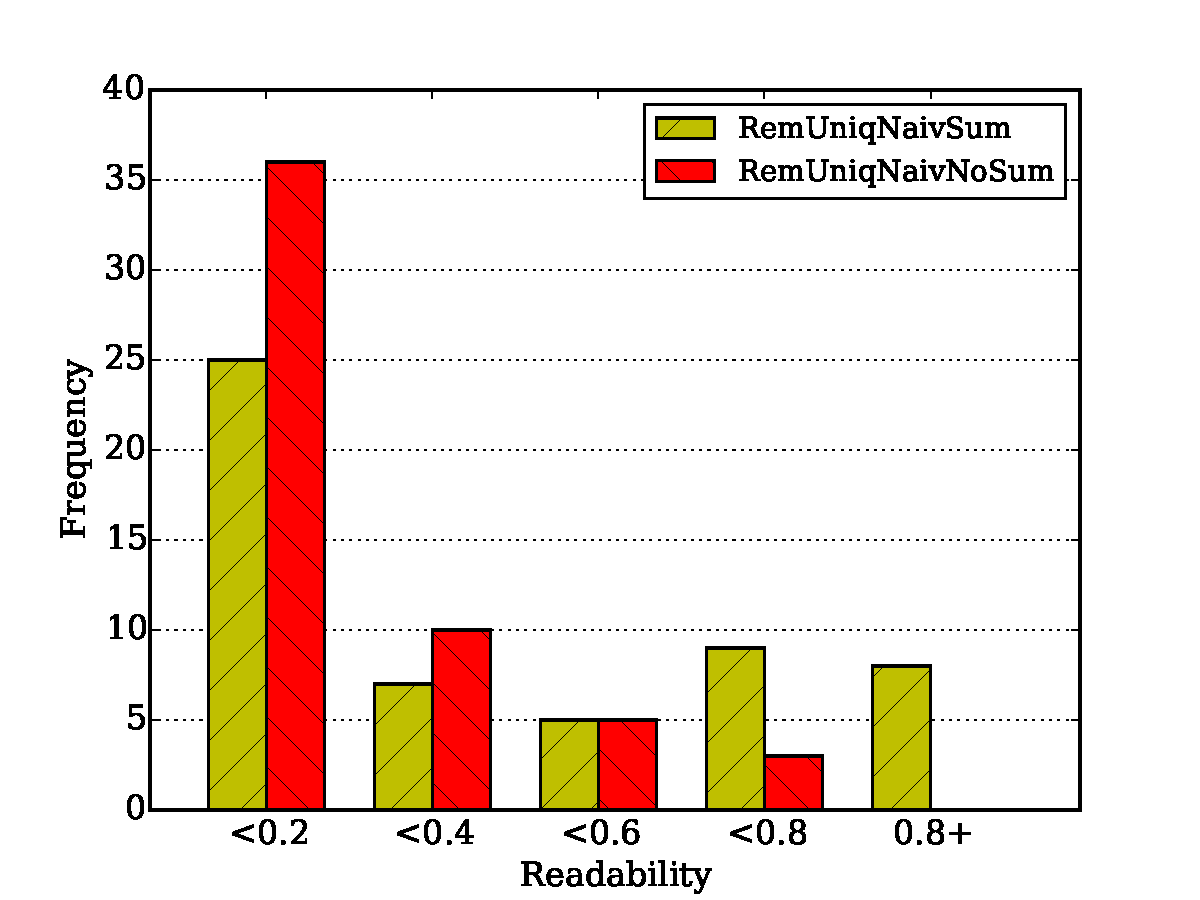
\includegraphics[width=0.45\textwidth]{results/exp1-readability.pdf}}
  \hspace{1em}%
  \ffigbox[\FBwidth]
    {\caption{}\label{res:exp1-plocs}}
    {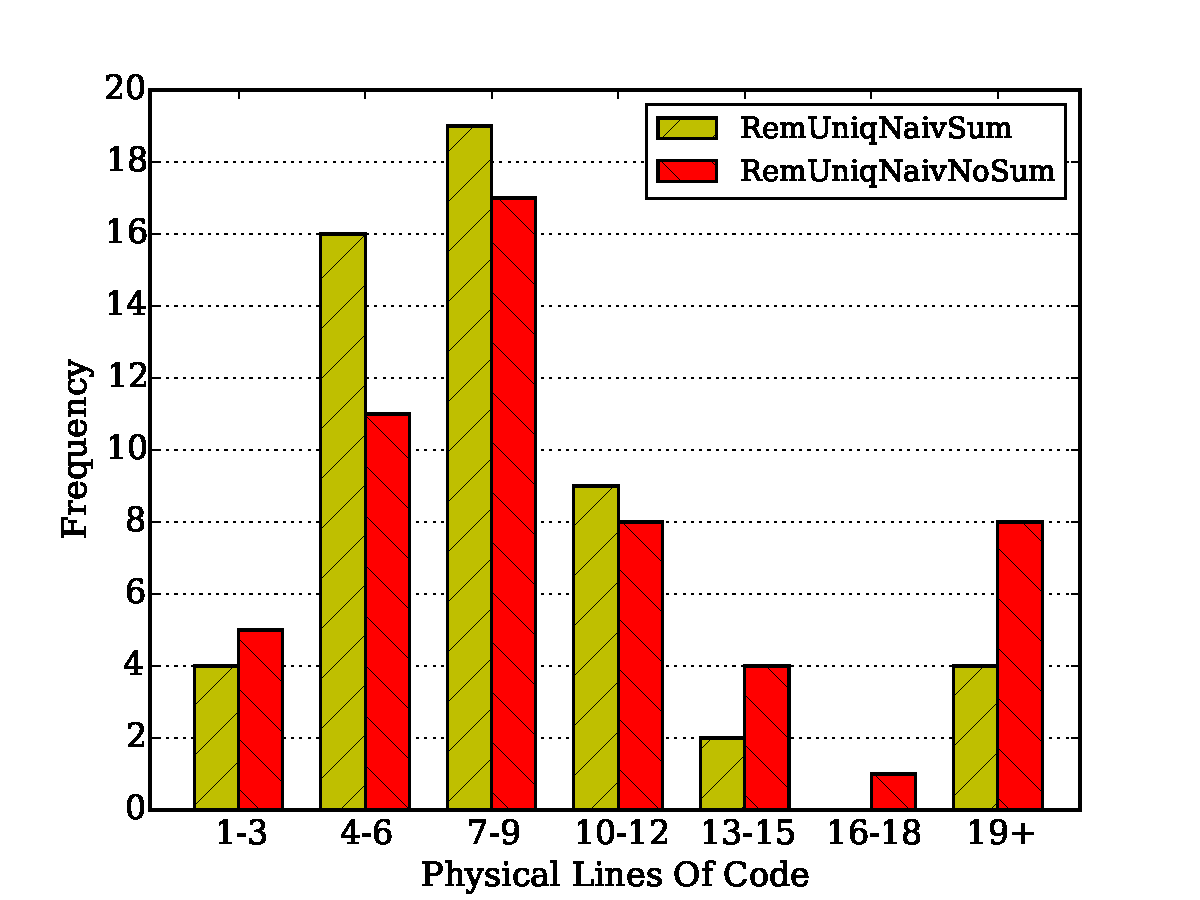
\includegraphics[width=0.45\textwidth]{results/exp1-plocs.pdf}}
  \end{subfloatrow}}
  {\caption[Illustration of the PLOCs, and the readability metrics\protect\\($RemUniqNaivNoSum$, $RemUniqNaivNoSum$)]{Figures illustrating (\subref{res:exp1-readability}) the readability distribution of the snippets, and (\subref{res:exp1-plocs}) the corresponding PLOCs distribution, for both versions of the system.}
\label{res:exp1-read-plocs}}
\end{figure}

In addition to the quantitative metrics and the plots presented in the last two sections, we present a few indicative mined snippets of the two versions in \Cref{sec:exp1-qualitative}.


\section{Experiment 2 - Evaluating the Preprocessing Step}
\label{sec:evaluation-exp2}

In the experiment of this section, we are going to investigate whether the removal of the unique sequences, during the preprocessing step, improves the results of the system. In order to do so we use the $RemUniqNaivSum$, as well as the $KeepUniqNaivSum$ versions of the system. In both of them the summariser is enabled, while they use the $naive$ clustering technique, where only identical sequences are clustered together. Although these two versions result to a quite different number of clusters, and to a different number of mined snippets consequently, the number of clusters is computed using the same methodology, based on the number of the non-identical sequences in each case. The hypothesis under evaluation is described below:

\begin{hypothesis}
Unique sequences often occur in handwritten examples, while removing them may additionally lead to limited coverage of the API.
\end{hypothesis}


\subsection{Quantitative results}
\label{subsec:evaluation-exp2-quantitative}

The removal of the unique sequences reduces the number of sequences to be clustered from $660$ to $175$. Then, the number of clusters identified by the naive clustering technique, in the $RemUniqNaivSum$ version, is $54$. On the other hand, the $KeepUniqNaivSum$ version, which does not remove the unique sequences, identifies $539$ clusters, using the naive clustering technique. This huge difference in the number of clusters reveals that the removal of the unique sequences may lead to limited snippets, which do not sufficiently cover the API.

\begin{table}[ht]
\centering
\small
\caption[Evaluation metrics\protect\\($RemUniqNaivSum$, $KeepUniqNaivSum$)]{Evaluation metrics for the version that removes the unique sequences ($RemUniqNaivSum$), and for this that does not remove them ($KeepUniqNaivSum$).}
\label{tables:evaluation-preprocessor}
\begin{tabular}{lll}
\toprule
Metric & $RemUniqNaivSum$ & $KeepUniqNaivSum$ \\
\midrule
$sequence\_precision$ & 0.28 & 0.14 \\
$snippet\_precision$ & 0.20 & 0.08 \\
$avg\_seq\_prec@50$ & \color{red}0.28 & \color{red}0.40 \\
$avg\_snip\_prec@50$  & 0.19 & 0.24 \\
$sequence\_nDCG_{50}$ & \color{red}0.34 & \color{red}0.42 \\
$snippet\_nDCG_{50}$  & 0.23 & 0.25 \\
$coverage\_of\_API\_methods$ & \color{red}14.53 & \color{red}88.63 \\
\bottomrule
\end{tabular}
\end{table}

Indeed, as shown in \Cref{tables:evaluation-preprocessor}, well less than $15\%$ of the API methods are covered by the snippets mined by the $RemUniqNaivSum$ version. This, compared to the fact that the handwritten examples cover around $38\%$ of the API methods, indicates that \textit{the removal of unique sequences actually leads to limited coverage of the API}.

As regards the number of snippets that match to handwritten examples, we find out that the $RemUniqNaivSum$ version includes $15$ of them, out of the $54$ mined in total. On the other hand, $73$ snippets out of the $520$ mined by the $KeepUniqNaivSum$ version match to at least one handwritten example. This shows that \textit{unique sequences often occur in handwritten examples}.

Looking at the precision metrics, we firstly present the $sequence\_precision$, and the $snippet\_precision$, which do not take into account the ranking, while they consider the total number of the results. However, a more fair comparison would take into consideration the same number of results for both versions. Such a comparison is possible using the next four metrics presented in \Cref{tables:evaluation-preprocessor}, which show that \textit{preserving the unique sequences does not only ensure a higher coverage in API methods, but it also ensures a higher precision among the top results}. We could claim that we expected such a behaviour, as the fact that a sequence is unique does not necessarily mean that it is not supported by other sequences; indeed, although a sequence may not be frequent on itself, it may be a subsequence of frequent sequences. In the latter case, the ranker plays a major role on the results of the metrics presented here, as it ranks the snippets based on their sequence's support in the dataset which, as explained in \Cref{sec:ranker}, takes into account its super-sequences.


\subsection{Visualising the Results}
\label{subsec:evaluation-exp2-plots}

The analytical results of the metrics presented in \Cref{tables:evaluation-preprocessor} are plotted in this subsection.

\Cref{res:exp2-calls-precision} indicates that it is quite possible that rare snippets -that contain unique sequences- exist in the \texttt{examples} directory. Although the relationship presented in this figure is not linear (it seems to be linear up to a threshold $k=100$), it still shows that unique snippets -with respect to their API call sequences- are often part of the documentation of an API. Moreover, \Cref{res:exp2-coverage} makes clear that, although the removal of unique sequences leads to higher coverage for the same value of $k$, up to a threshold (e.g. $k=50$), this results to limited coverage of the API methods in general, for larger values of $k$.

Regarding the precision metrics, we illustrate the precision at top $k$ in \Cref{res:exp2-precisionatk}, and the $nDCG_k$ in \Cref{res:exp2-ndcg}, for both the snippets and their associated sequences. An interesting point shown in all these figures is that the $RemUniqNaivSum$ version seems to ensure only a limited number ($\leq 25$) of high quality results, in terms of their precision to the handwritten examples. That is, if we were only interested in e.g. the top $20$ snippets of the API, then probably this version could mine sufficient snippets of high precision. However, we believe that this number would only be acceptable for someone who is looking for a limited number of the top snippets of an API, rather than on snippets that contain specific methods or classes of the API.

\begin{figure}[H]
\ffigbox
{%
  \begin{subfloatrow}[2]
  \ffigbox[\FBwidth]
    {\caption{}\label{res:exp2-calls-precision}}
    {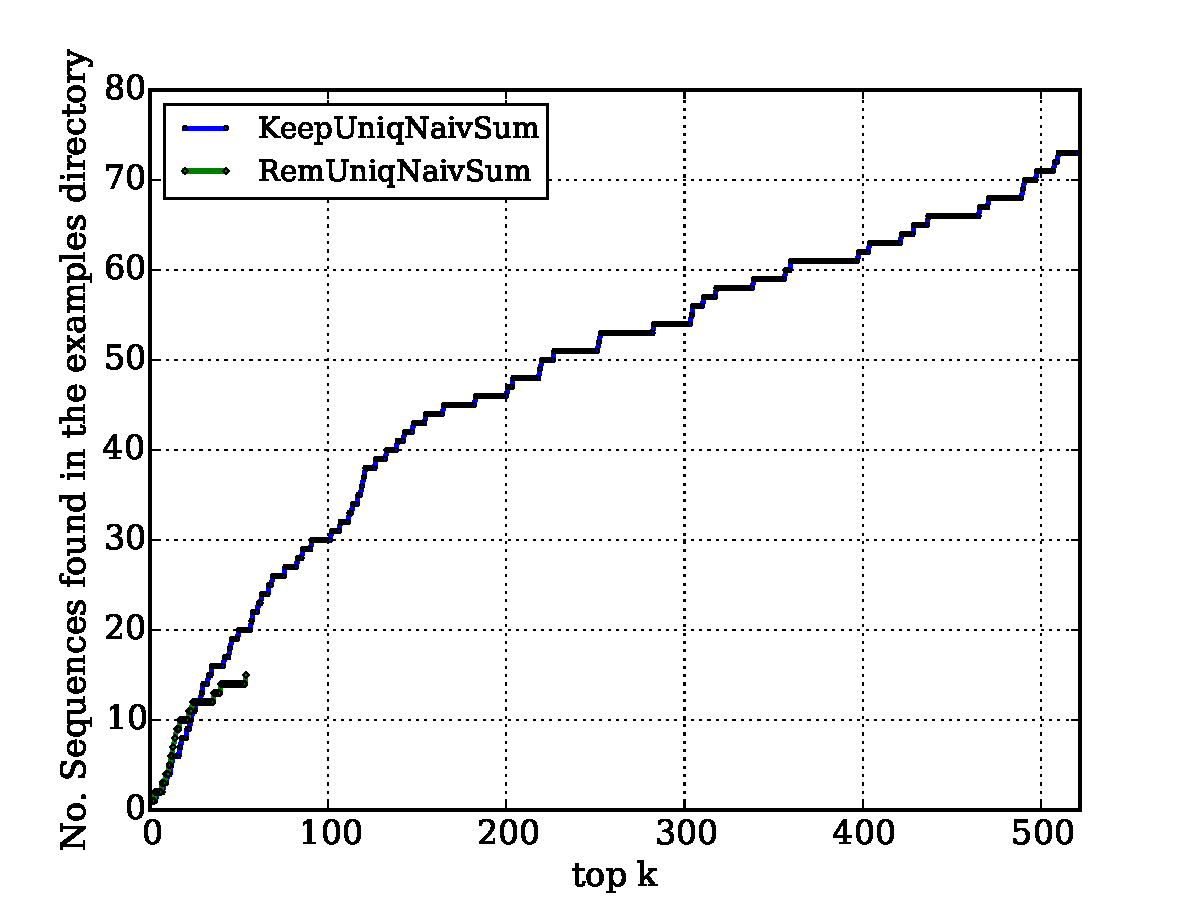
\includegraphics[width=0.45\textwidth]{results/exp2-calls-precision.pdf}}
  \hspace{1em}%
  \ffigbox[\FBwidth]
    {\caption{}\label{res:exp2-coverage}}
    {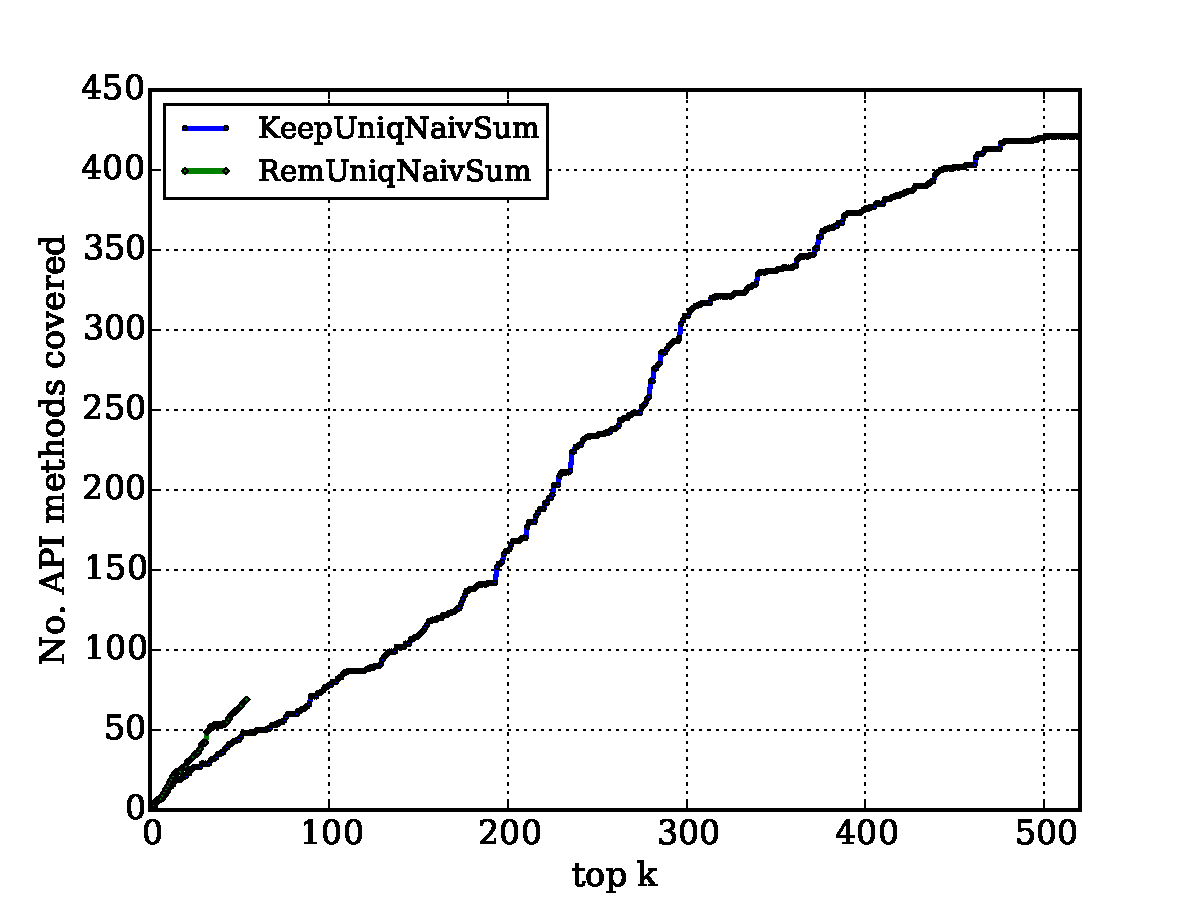
\includegraphics[width=0.45\textwidth]{results/exp2-coverage.pdf}}
  \end{subfloatrow}}
  {\caption[Illustration of the precision and coverage\protect\\($RemUniqNaivSum$, $RemUniqNaivSum$)]{Figures illustrating (\subref{res:exp2-calls-precision}) the number of snippets whose sequences match to at least one example, and (\subref{res:exp2-coverage}) the number of API methods covered by the mined snippets, using the top $k$ mined snippets for both versions.}
\label{res:exp2-calls-prec-coverage}}
\end{figure}

\vspace{-20pt}

\begin{figure}[H]
\ffigbox
{%
  \begin{subfloatrow}[2]
  \ffigbox[\FBwidth]
    {\caption{}\label{res:exp2-sequence-precision}}
    {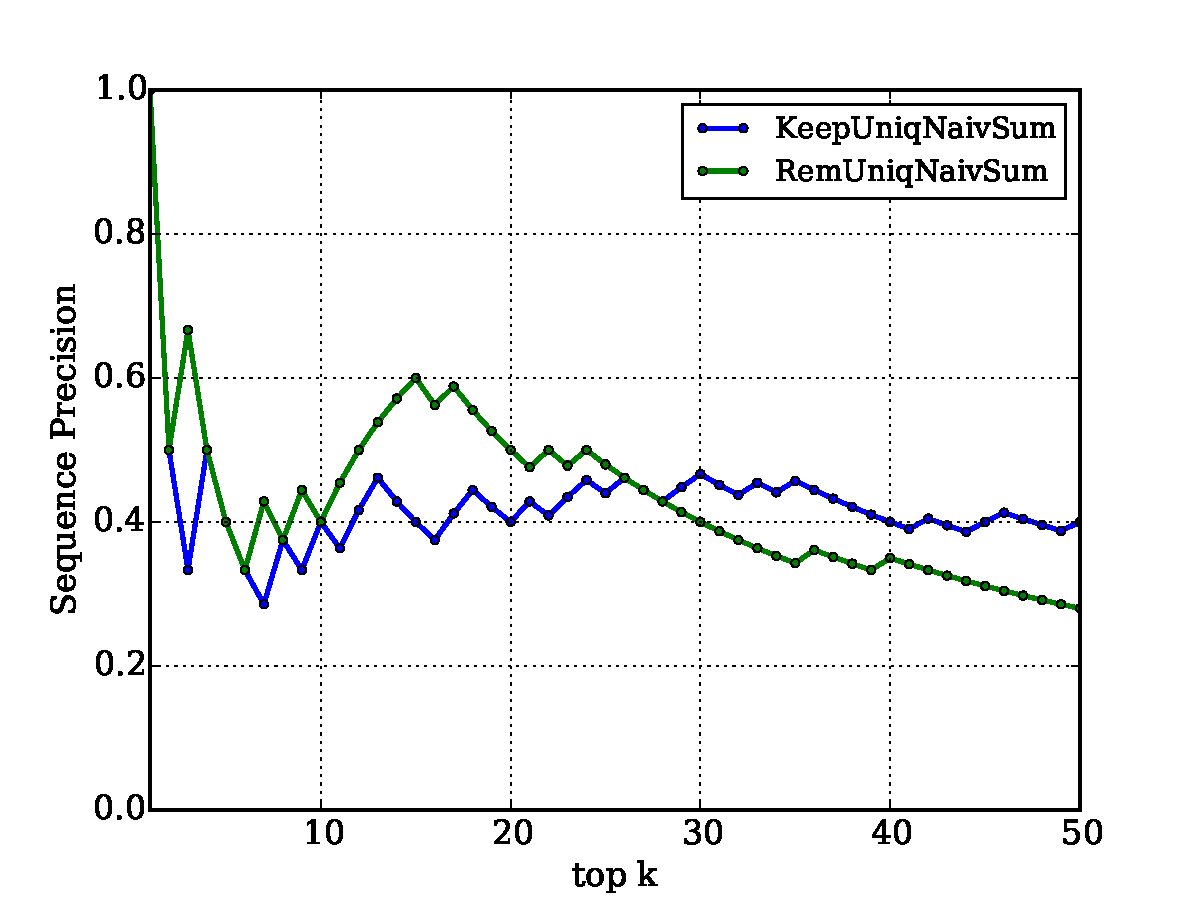
\includegraphics[width=0.45\textwidth]{results/exp2-sequence-precision.pdf}}
  \hspace{1em}%
  \ffigbox[\FBwidth]
    {\caption{}\label{res:exp2-snippet-precision}}
    {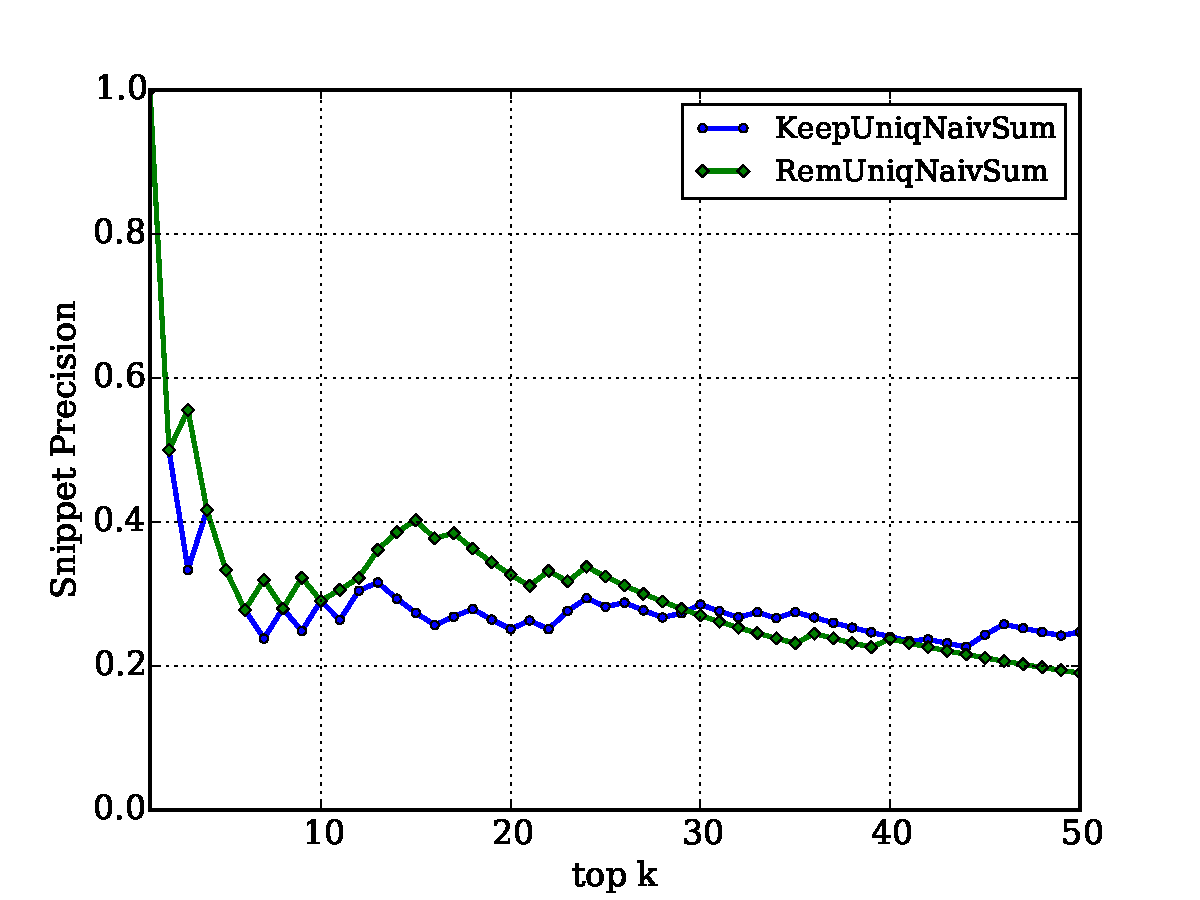
\includegraphics[width=0.45\textwidth]{results/exp2-snippet-precision.pdf}}
  \end{subfloatrow}}
  {\caption[Illustration of the precision at top $k$\protect\\($RemUniqNaivSum$, $RemUniqNaivSum$)]{Figures illustrating (\subref{res:exp2-sequence-precision}) the sequence precision, and (\subref{res:exp2-snippet-precision}) the snippet precision at top $k$, for both versions.}
\label{res:exp2-precisionatk}}
\end{figure}

\vspace{-20pt}

\begin{figure}[H]
\ffigbox
{%
  \begin{subfloatrow}[2]
  \ffigbox[\FBwidth]
    {\caption{}\label{res:exp2-sequence-ndcg}}
    {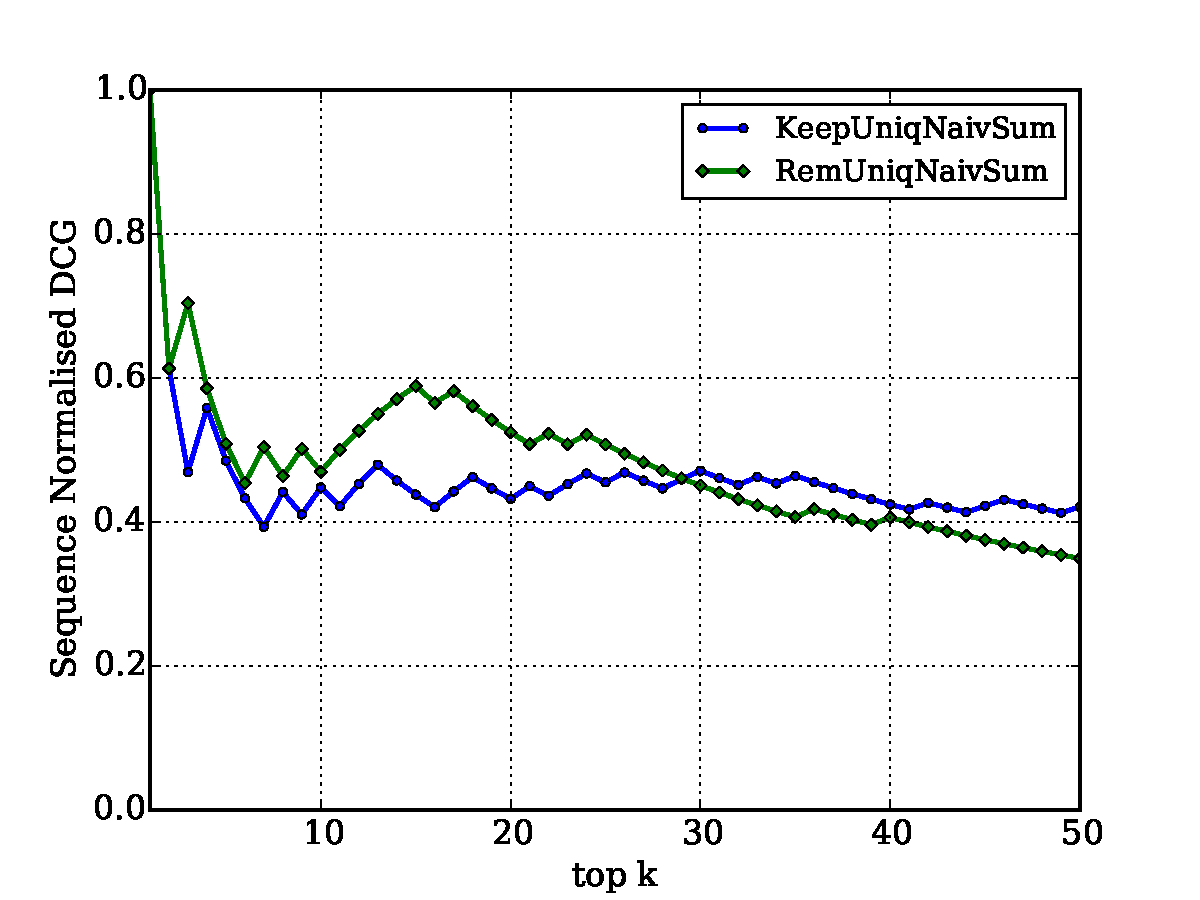
\includegraphics[width=0.45\textwidth]{results/exp2-sequence-ndcg.pdf}}
  \hspace{1em}%
  \ffigbox[\FBwidth]
    {\caption{}\label{res:exp2-snippet-ndcg}}
    {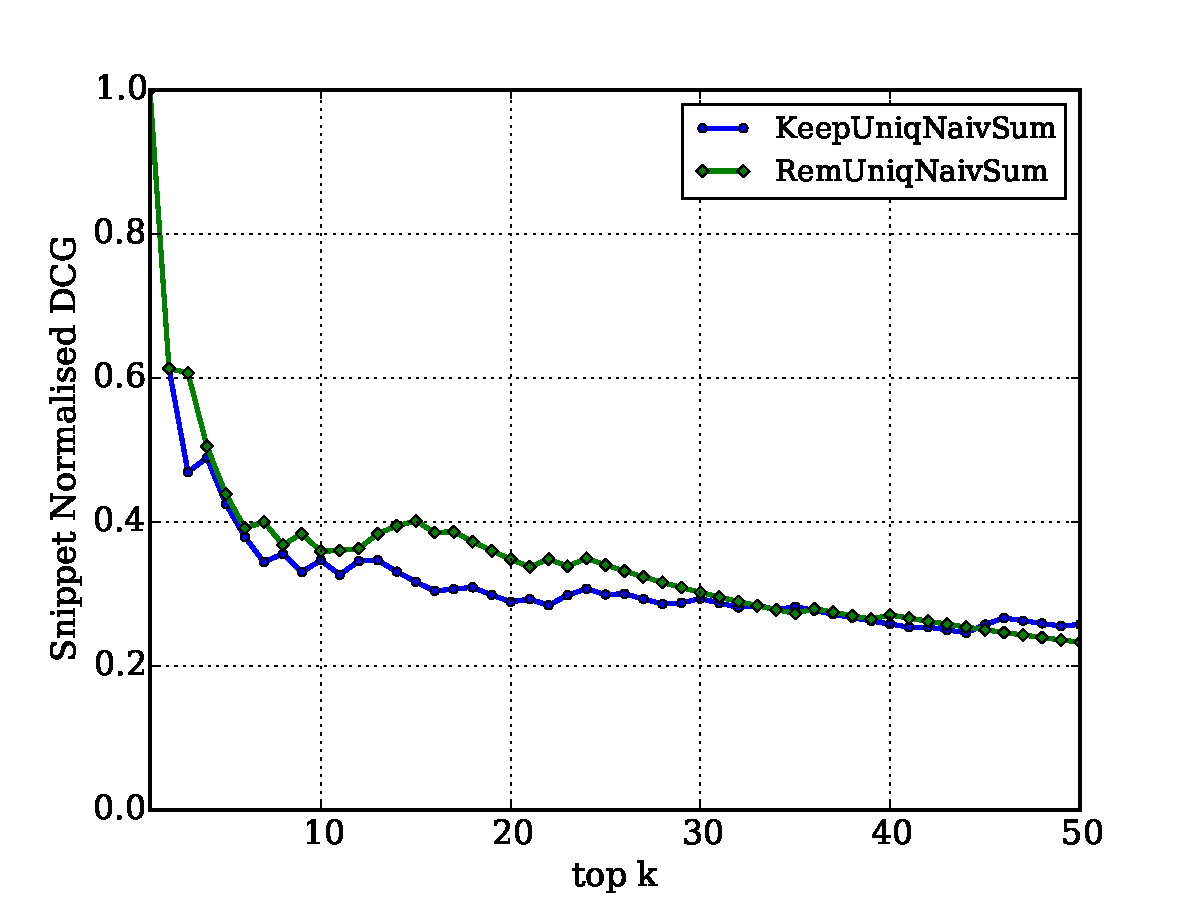
\includegraphics[width=0.45\textwidth]{results/exp2-snippet-ndcg.pdf}}
  \end{subfloatrow}}
  {\caption[Illustration of the $nDCG_k$ metric\protect\\($RemUniqNaivSum$, $RemUniqNaivSum$)]{Figures illustrating (\subref{res:exp2-sequence-ndcg}) the $sequece\_nDCG_k$, and (\subref{res:exp2-snippet-ndcg}) the $snippet\_nDCG_k$, for both versions.}
\label{res:exp2-ndcg}}
\end{figure}
\vspace{-30pt}

\section{Experiment 3 - Evaluating the Clustering Techniques}
\label{sec:evaluation-exp3}

In the following experiment, we are going to investigate whether the application of different clustering techniques leads to different results. For this purpose we make use of the $KeepUniqKMedoidsSum$, as well as of the $KeepUniqHDBSCANSum$ versions of the system. Both of them preserve the unique sequences in the preprocessing step, while they leverage the summariser. In order for the comparison between the $k$-medoids and the HDBSCAN algorithm to be fair, we use the same number of clusters for both of them. In order to ensure this, we set the $min\_cluster\_size$ parameter of the HDBSCAN algorithm to $2$, which leads to $110$ clusters for the \texttt{Twitter4J} API. Then, we use the same number of clusters for the $k$-medoids algorithm. The hypothesis under evaluation is described below:

\begin{hypothesis}
Different clustering techniques lead to similar clusterings, and mined snippets consequently, for the same number of clusters.
\end{hypothesis}

The first part of the hypothesis could be evaluated based on qualitative examples, as well as based on clustering evaluation metrics. However, we are mainly interested in the second part of the hypothesis. This means that, even though the clusters formed by a clustering technique may be characterised by low \textit{cohesion} and \textit{separation}, or even \textit{silhouette coefficient} values, the technique may lead to valuable mined snippets.


\subsection{Quantitative Results}
\label{subsec:evaluation-exp3-quantitative}

Evaluating the algorithms using clustering evaluation metrics, we find out that the clusterings of both algorithms show a quite low silhouette coefficient value. More specifically, the silhouette score for the $KeepUniqKMedoidsSum$ version is $0.13$, while the corresponding score for the $KeepUniqHDBSCANSum$ is even lower ($<0.1$). However, this is an effect of the quite noisy data, which prompts us to avoid using popular clustering evaluation metrics, for the evaluation of this part of the system. After all, based on this experiment's hypothesis, we are mainly interested on whether different clustering techniques lead to different clusterings and mined snippets, rather than on evaluating the quality of the clusters.

\Cref{tables:evaluation-clustering} presents the metrics used in order to decide on whether the different clustering techniques result to different mined snippets. At first, we see that the sequence-based precision metrics do not show any real difference. The HDBSCAN algorithm seems to perform slightly better than the $k$-medoids algorithm, however, the difference between the two algorithms is negligible enough to proceed to such a conclusion. In addition to that, both versions achieve similar coverage of the API. These two facts indicate that the two clustering techniques mine similar sequences. Indeed, the reader may find the top 10 sequences, with respect to their support in the dataset, mined by the two algorithms, in \Cref{sec:exp3-qualitative}, where it is shown that there is only a slight difference between the sequences mined by the two versions.

\begin{table}[ht]
\centering
\small
\caption[Evaluation metrics\protect\\($KeepUniqKMedoidsSum$, $KeepUniqHDBSCANSum$)]{Evaluation metrics for the version that uses the $k$-medoids clustering technique, and for that which uses the HDBSCAN algorithm.}
\label{tables:evaluation-clustering}
\begin{tabular}{lll}
\toprule
Metric & $KeepUniqKMedoidsSum$ & $KeepUniqHDBSCANSum$ \\
\midrule
$sequence\_precision$ & \color{red}0.17 & \color{red}0.20 \\
$snippet\_precision$ & 0.11 & 0.12 \\
$matched\_snippet\_precision$ & 0.65 & 0.62 \\
$sequence\_nDCG_{110}$ & \color{red}0.25 & \color{red}0.26 \\
$snippet\_nDCG_{110}$  & 0.16 & 0.16 \\
$coverage\_of\_API\_methods$ & \color{red}37.47 & \color{red}39.80 \\
\bottomrule
\end{tabular}
\end{table}

We also present the snippet-based precision metrics in \Cref{tables:evaluation-clustering}, although these are not really relevant to this experiment, as the clustering techniques take into account only the API call sequences of the files, and not their source code, which is considered at a later stage.


\subsection{Visualising the Results}
\label{subsec:evaluation-exp3-plots}

The analytical results of the sequence-based metrics presented in \Cref{tables:evaluation-clustering} are plotted in this subsection.

\begin{figure}[t]
\ffigbox
{%
  \begin{subfloatrow}[2]
  \ffigbox[\FBwidth]
    {\caption{}\label{res:exp3-calls-precision}}
    {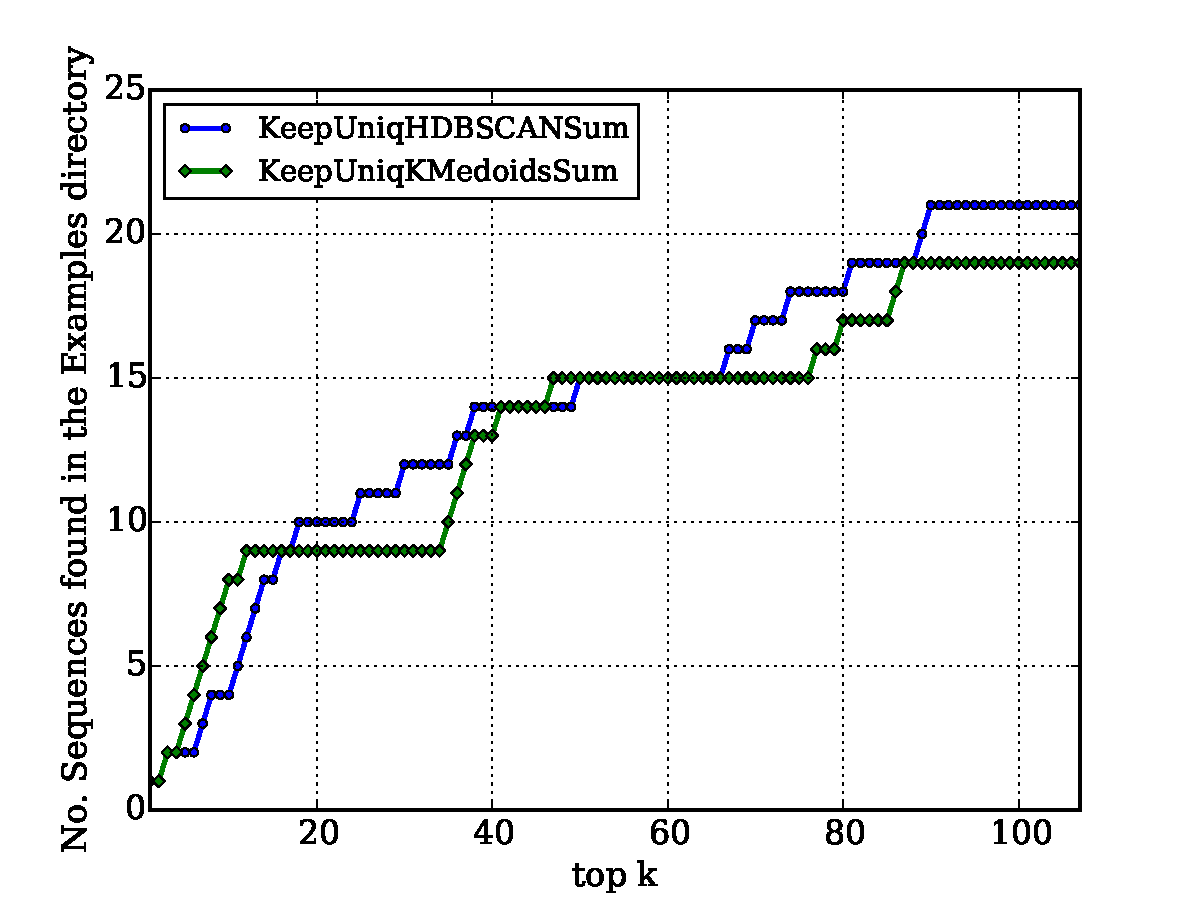
\includegraphics[width=0.45\textwidth]{results/exp3-calls-precision.pdf}}
  \hspace{1em}%
  \ffigbox[\FBwidth]
    {\caption{}\label{res:exp3-coverage}}
    {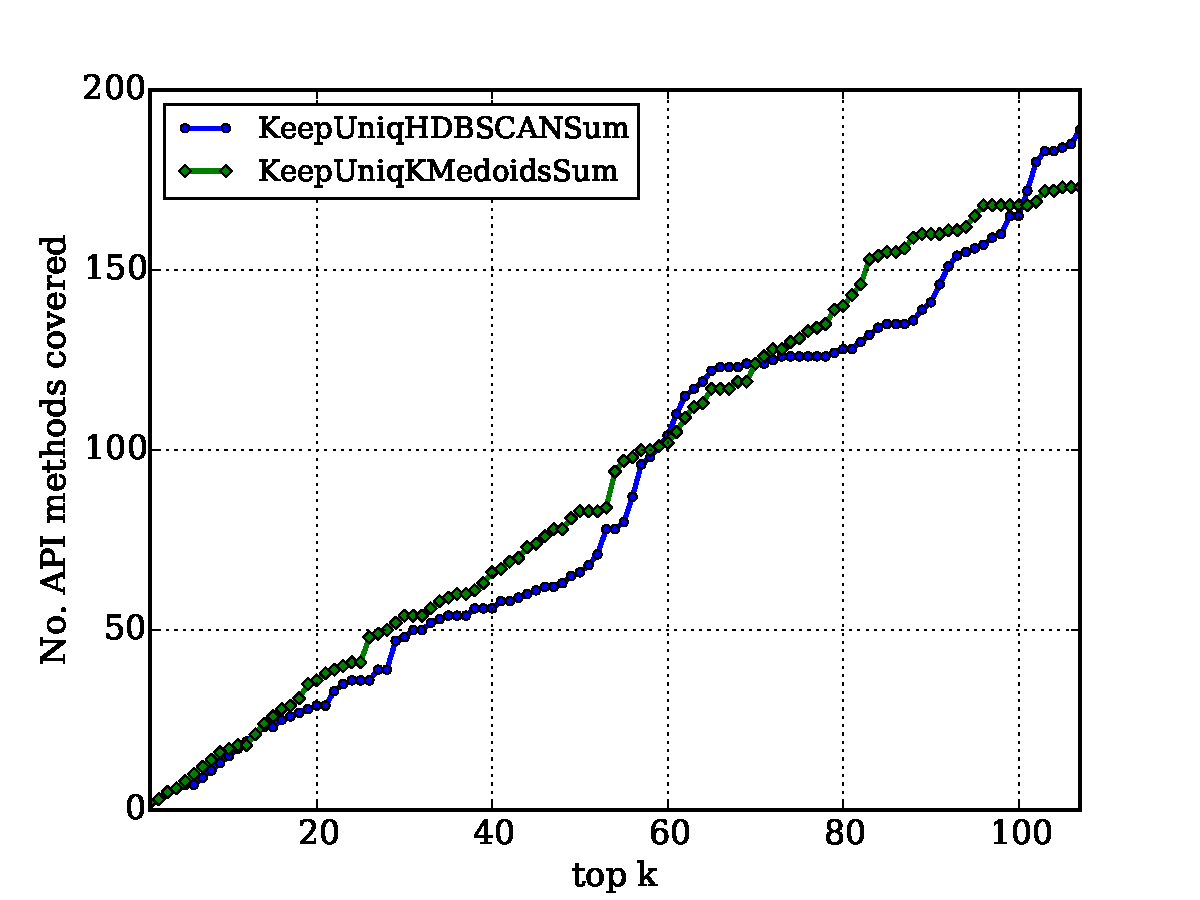
\includegraphics[width=0.45\textwidth]{results/exp3-coverage.pdf}}
  \end{subfloatrow}}
  {\caption[Illustration of the precision and coverage\protect\\($KeepUniqKMedoidsSum$, $KeepUniqHDBSCANSum$)]{Figures illustrating (\subref{res:exp3-calls-precision}) the number of snippets whose sequences match to at least one example, and (\subref{res:exp3-coverage}) the number of API methods covered by the mined snippets, using the top $k$ mined snippets, for both versions.}
\label{res:exp3-calls-prec-coverage}}
\end{figure}

As depicted in \Cref{res:exp3-calls-prec-coverage}, the number of sequences found in the handwritten examples follows a similar trend for both versions, while the same number of methods are being covered by the two versions, for similar $k$ values. Combining these plots with the metrics presented in the previous section, we see that the two clustering techniques lead to similar clusterings\footnote{A better interpretation is that both clustering techniques lead to similar clusters' centres, as actually the clusters' centres are used in order to mine a sequence from each cluster and then retrieve its source code file.}.

\begin{figure}
\ffigbox
{%
  \begin{subfloatrow}[2]
  \ffigbox[\FBwidth]
    {\caption{}\label{res:exp3-sequence-precision}}
    {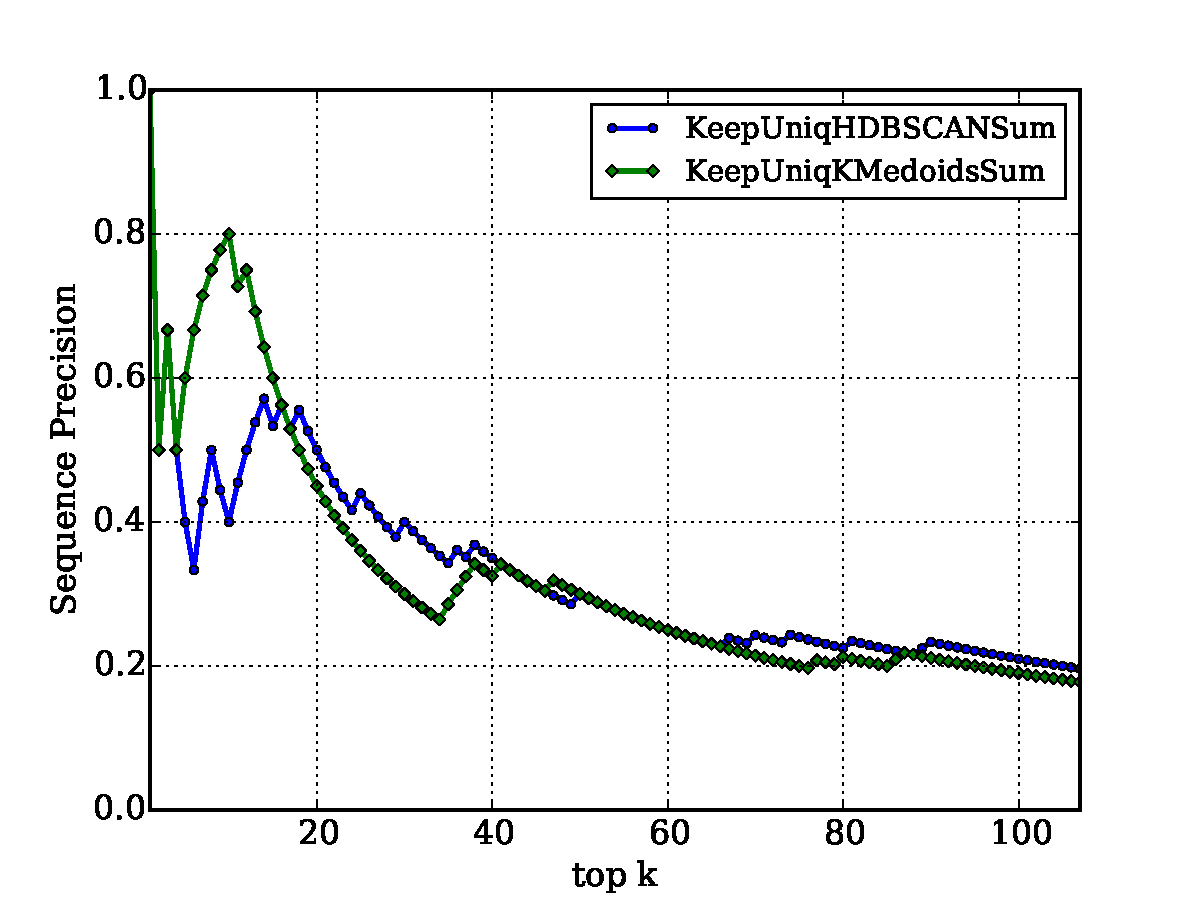
\includegraphics[width=0.45\textwidth]{results/exp3-sequence-precision.pdf}}
  \hspace{1em}%
  \ffigbox[\FBwidth]
    {\caption{}\label{res:exp3-sequence-ndcg}}
    {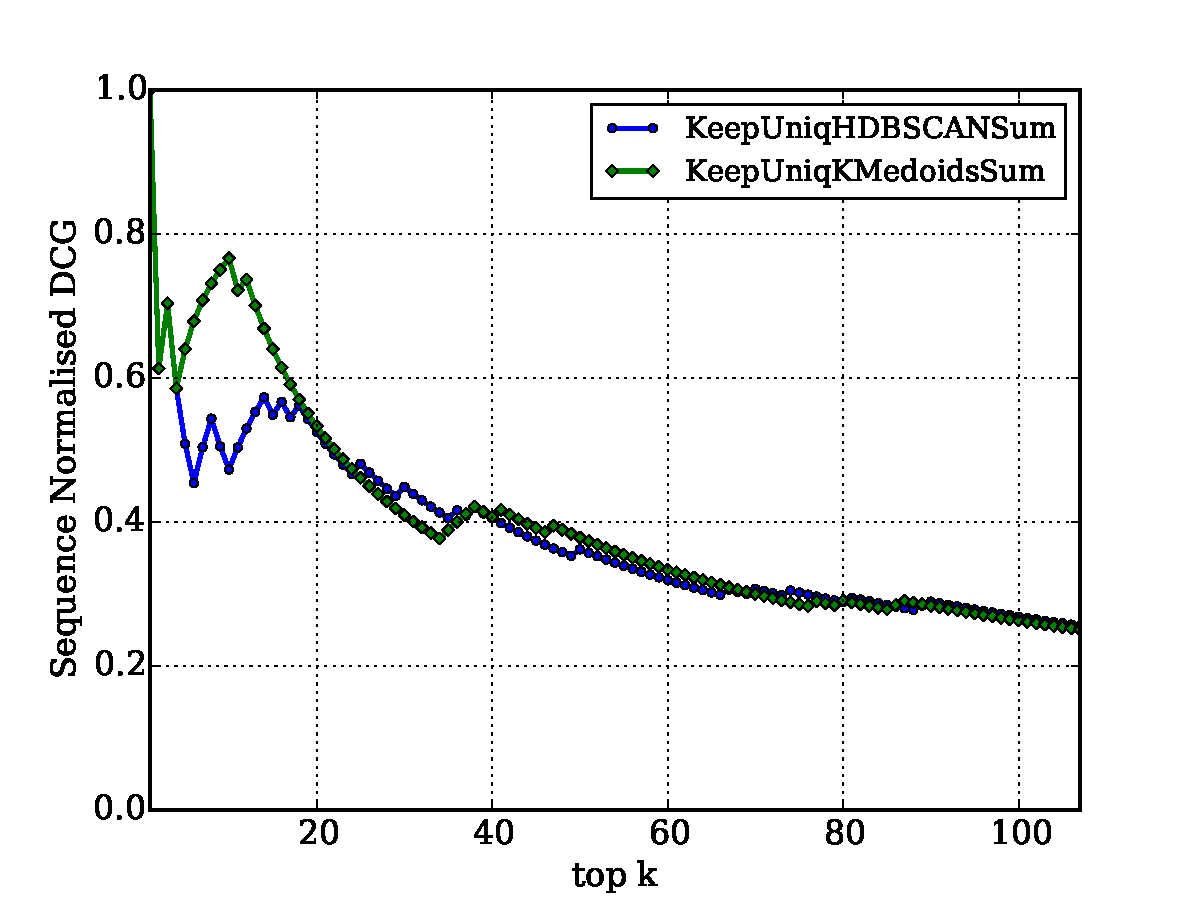
\includegraphics[width=0.45\textwidth]{results/exp3-sequence-ndcg.pdf}}
  \end{subfloatrow}}
  {\caption[Illustration of the precision at top $k$, and the $nDCG_k$ metrics\protect\\($KeepUniqKMedoidsSum$, $KeepUniqHDBSCANSum$)]{Figures illustrating (\subref{res:exp3-sequence-precision}) the sequence precision at top $k$, and (\subref{res:exp3-sequence-ndcg}) the $sequence\_nDCG_k$, for both versions.}
\label{res:exp3-precision-ndcg}}
\end{figure}

\Cref{res:exp3-precision-ndcg} shows a slightly increased sequence precision, for the $k$-medoids version, for the top $20$ sequences. However, after a manual inspection, we find out that this can be explained as follows; the top sequences of the HDBSCAN algorithm are more complex sequences than these mined by the $k$-medoids technique, containing more than two API calls. Moreover, checking the support of these sequences, we surprisingly find out that the sequences mined by the $k$-medoids algorithm have lower support than these mined by the HDBSCAN technique. This interesting point, combined with all the previous results shown in this experiment leads us to one more conclusion; it is quite hard to determine on the best clustering technique for systems that conduct API mining, without having an indication of the system's results, with respect to the handwritten examples.

Taking into account that there is no real difference between the two clustering techniques, we could claim that the HDBSCAN algorithm seem a more preferable solution, as this algorithm is almost parameter-free. This is based on the fact that we could, in any case, set the $min\_cluster\_size$ parameter to $2$, and the algorithm would then estimate the number of clusters.


\section{Experiment 4 - Comparing Naive with Powerful Clustering Techniques}
\label{sec:evaluation-exp4}

In the experiment presented in this section, we are going to investigate whether the application of clustering techniques that cluster similar rather than identical sequences improves the results. For this purpose we use the $KeepUniqNaiveSum$, as well as the $KeepUniqKMedoidsSum$, and the $KeepUniqHDBSCANSum$ versions of the system. The first version clusters only identical sequences, and leads to a large number of clusters, while the other two versions cluster similar sequences, and output the most representative ones, thus leading to less clusters. Similarly to the previous example, we use the same number of clusters for the $KeepUniqKMedoidsSum$ and the $KeepUniqHDBSCANSum$ versions ($k=110$). The hypothesis under evaluation is described below:

\begin{hypothesis}
More powerful clustering techniques, that cluster similar rather than identical sequences, lead to more valuable snippets.
\end{hypothesis}

We believe that an efficient way in order to evaluate the hypothesis, is to plot the precision against the coverage of the API, in a similar manner to that used in the precision against recall figures. Such an illustration would reveal the value of the snippets to the developers. That is, if a system mines snippets that are precise and cover a large part of the API concurrently, then this system would be of great value to the developers.

A common way in order to eliminate the saw-tooth shape of the precision against recall curve, is to plot the \textit{interpolated precision against recall curve}, where the highest precision found for any recall value (or level) $\geq$ current recall is shown\footnote{\url{http://nlp.stanford.edu/IR-book/html/htmledition/evaluation-of-ranked-retrieval-results-1.html}}. In our case, we use the same concept in order to plot the precision against coverage curve. In such a plot, the curve shows a decreasing trend and facilitates the drawing of possible conclusions.

\begin{figure}
\ffigbox
{%
  \begin{subfloatrow}[2]
  \ffigbox[\FBwidth]
    {\caption{}\label{res:exp4-interp-prec-cov50}}
    {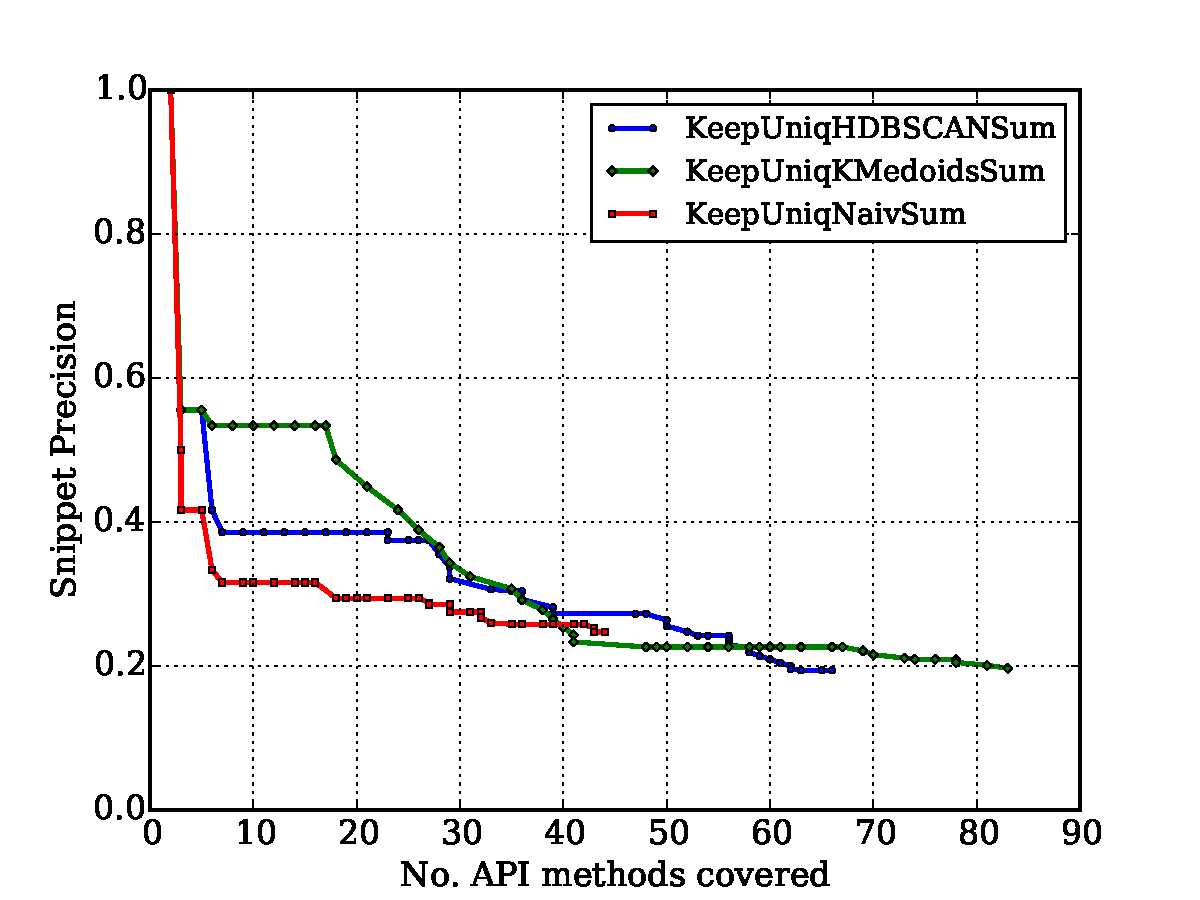
\includegraphics[width=0.45\textwidth]{results/exp4-interp-prec-cov50.pdf}}
  \hspace{1em}%
  \ffigbox[\FBwidth]
    {\caption{}\label{res:exp4-interp-prec-cov100}}
    {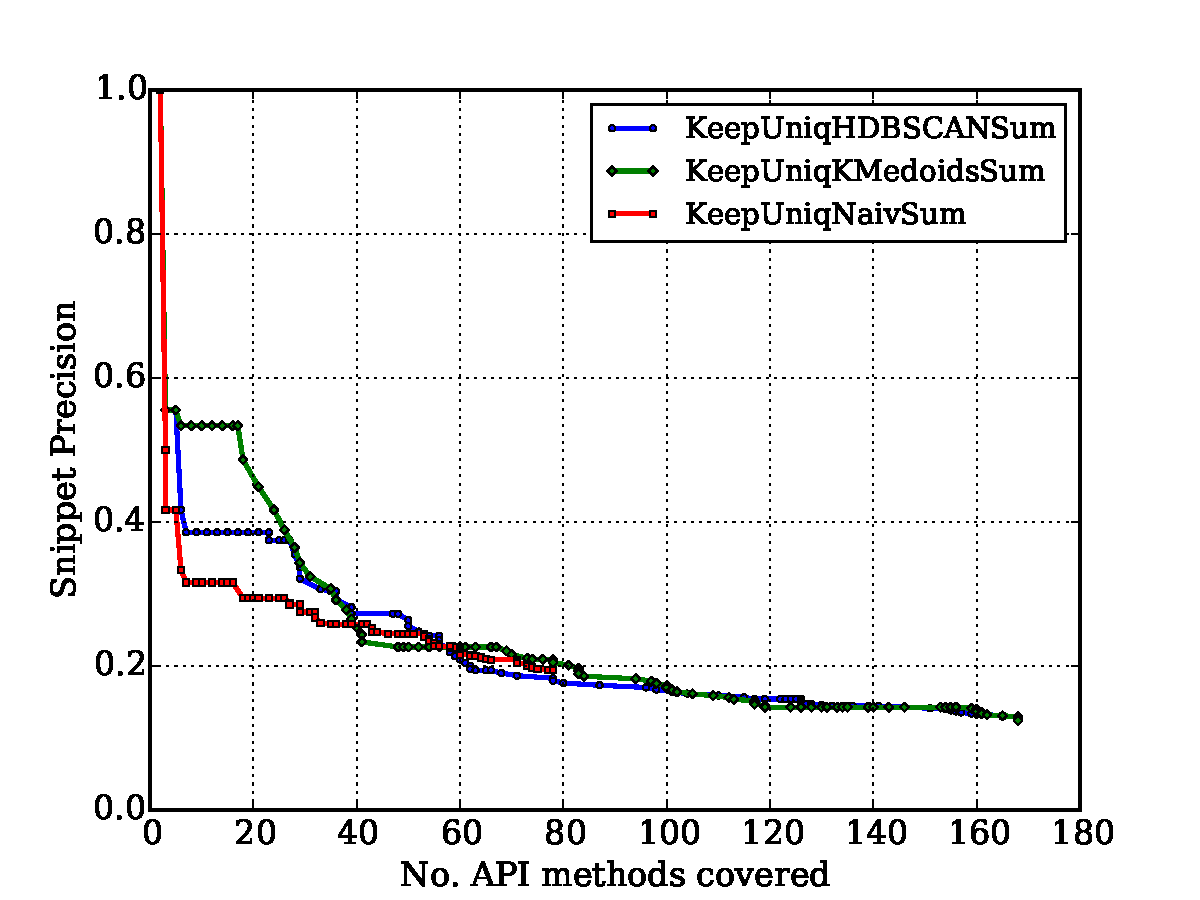
\includegraphics[width=0.45\textwidth]{results/exp4-interp-prec-cov100.pdf}}
  \end{subfloatrow}}
  {\caption[Illustration of the average interpolated precision against coverage\protect\\($KeepUniqNaiveSum$, $KeepUniqKMedoidsSum$,\protect\\$KeepUniqHDBSCANSum$)]{Figures illustrating the average interpolated snippet precision against the API methods coverage for three different versions of the system, that leverage different clustering techniques (\subref{res:exp4-interp-prec-cov50}) using their top $50$ mined snippets, and (\subref{res:exp4-interp-prec-cov100}) using the top $100$ mined snippets.}
\label{res:exp4-interp-prec-cov}}
\end{figure}

In \Cref{res:exp4-interp-prec-cov50} we illustrate the precision against coverage of the API for the top $50$ mined snippets, while \Cref{res:exp4-interp-prec-cov100} is generated using the top $100$ mines snippets, and is obviously an extension of \Cref{res:exp4-interp-prec-cov50}. It is noteworthy to say that being up and to the right is better.

These plots seem really interesting. The coverage in API methods, achieved by the $KeepUniqNaiveSum$ version is quite low, which is related to the fact that this version clusters only identical sequences together. This means that it contains several similar snippets that use the same API calls (which is an indication of a high cohesion and a low separation). On the other hand, the $KeepUniqKMedoidsSum$ and the $KeepUniqHDBSCANSum$ versions achieve the best results here, and this indicates that there is a high separation between the clusters. More specifically, the $KeepUniqKMedoidsSum$ version achieves way better results for the first $25$ methods covered, as shown in \Cref{res:exp4-interp-prec-cov50}. This increased precision has been explained in the previous experiment, but here we also notice a difference in the methods covered, where the $KeepUniqKMedoidsSum$ version covers almost 85 API methods in its top $50$ mines snippets, with the $KeepUniqHDBSCANSum$ version covering well less than $65$, for the same value of $k$. However, this difference seems to be eliminated in \Cref{res:exp4-interp-prec-cov100}, which leads us to the conclusion that the $KeepUniqKMedoidsSum$ version performs better than the $KeepUniqHDBSCANSum$ version for smaller values of $k$.

In conclusion, this experiment indicates that the application of a clustering technique that clusters similar rather than identical sequences, leads to a better trade-off between the precision and coverage metrics which, in its turn, shows that \textit{the mined snippets of more powerful clustering techniques are of greater value to the developers}.


\section{Experiment 5 - Evaluating the Presentation of Snippets Rather Than of Sequences}
\label{sec:evaluation-exp5}

In this experiment we are going to investigate the key hypothesis of the current dissertation, which is that an API miner that presents snippets rather than sequences may help the users learn the target API easier. The hypothesis under evaluation is described below:

\begin{hypothesis}
Snippets are more useful to developers than sequences of API calls.
\end{hypothesis}

In an attempt to evaluate the hypothesis, we are going to make use of the\\$KeepUniqHDBSCANSum$ version of the system, although the clustering technique does not play a key role in this evaluation. The evaluation metric that would help us to conclude is the $addit\_snippet\_info$ one, which computes the additional information, in terms of tokens, that is shown to the users, when presenting snippets instead of sequences.

Computing the value of this metric for the total number of the results ($110$ results), we find that the ratio between the snippets-tokens and the sequence-tokens, that are shared between the mined snippets and their associated examples, is $3.4$. This means that the presentation of snippets instead of sequences leads to $3.4$ times more information to the developers. This value is noticeably high, especially if we take into account that we have not used any techniques in order to predict identifier names, which would lead to more common snippet-tokens between the mined snippets and their associated examples.

Plotting the additional information revealed by the snippets in \Cref{res:exp5-additional-info} (this is coloured green) we see that, almost in any case, presenting snippets instead of sequences reveals at least twice as much valuable information as this revealed by the sequences. More interestingly, there are even cases where the number of common tokens between a mined snippet and its associated example have been increased by eight times (e.g. in \textit{Snippet id}$=12$), when the presentation of the associated sequences would only reveal a few common tokens (less than $4$ in the usual case). 

In addition to \Cref{res:exp5-additional-info}, we also illustrate the distribution of the common tokens between the snippets and their associated examples, when these are presented as snippets and as API call sequences, in \Cref{res:exp5-common-tokens}. This figure makes clear that the presentation of sequences leads to limited information about the usage of the API, concealing valuable information, which can be revealed when presenting snippets. It is quite interesting that there are mined snippets with more than 15 common tokens with their associated examples. 

Furthermore, we present two indicative mined snippets in \Cref{sec:exp5-qualitative}, which show the additional information revealed when presenting snippets, as well as the power of our system to mine snippets that do not exist in the \texttt{examples} directory, which are however valuable.

Indubitably, both plots show that \textit{much more information is revealed when presenting snippets instead of sequences}. This conclusion confirms our initial hypothesis, while it also shows that \textit{our system successfully mines snippets that are valuable to the users, facilitating the use of the target API}.   

\begin{figure}[t]
\ffigbox
{%
  \begin{subfloatrow}[2]
  \ffigbox[\FBwidth]
    {\caption{}\label{res:exp5-additional-info}}
    {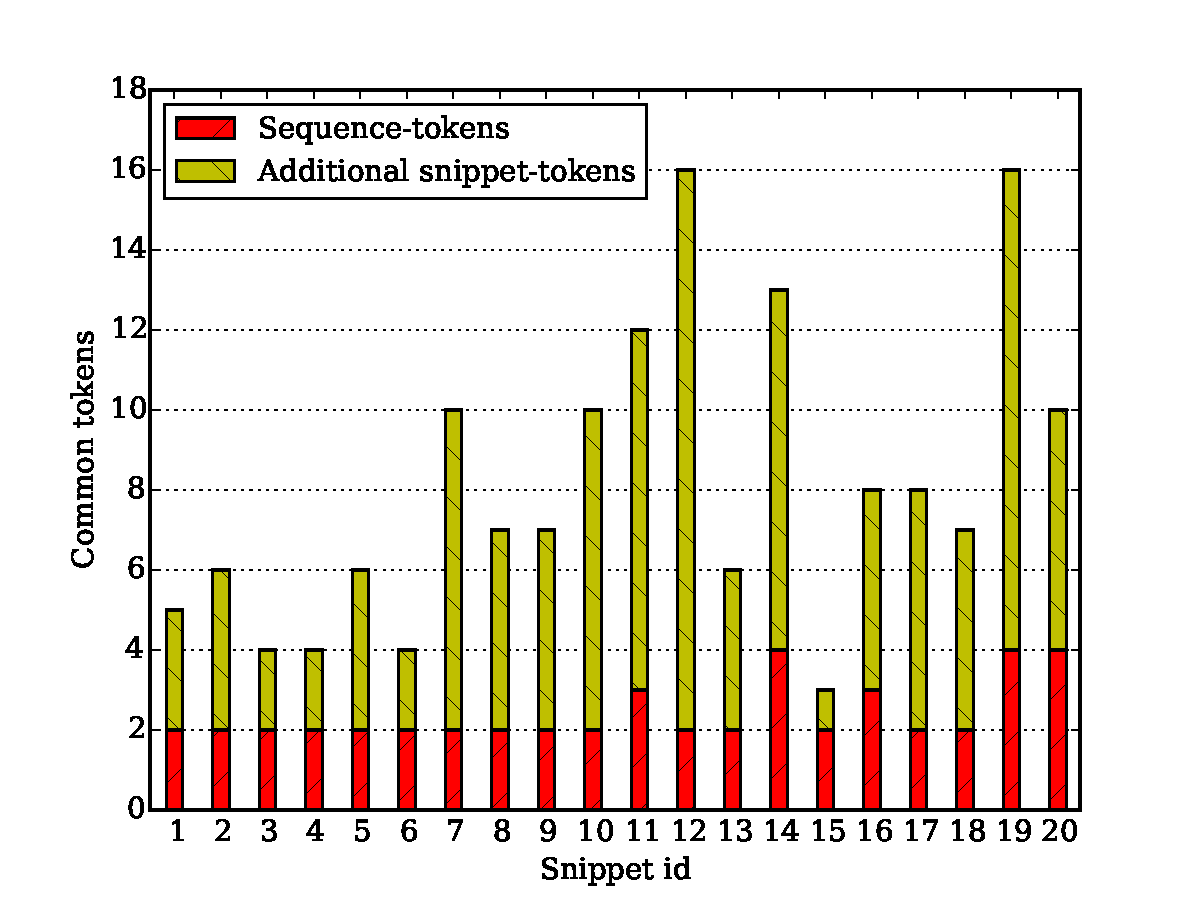
\includegraphics[width=0.45\textwidth]{results/exp5-additional-info.pdf}}
  \hspace{1em}%
  \ffigbox[\FBwidth]
    {\caption{}\label{res:exp5-common-tokens}}
    {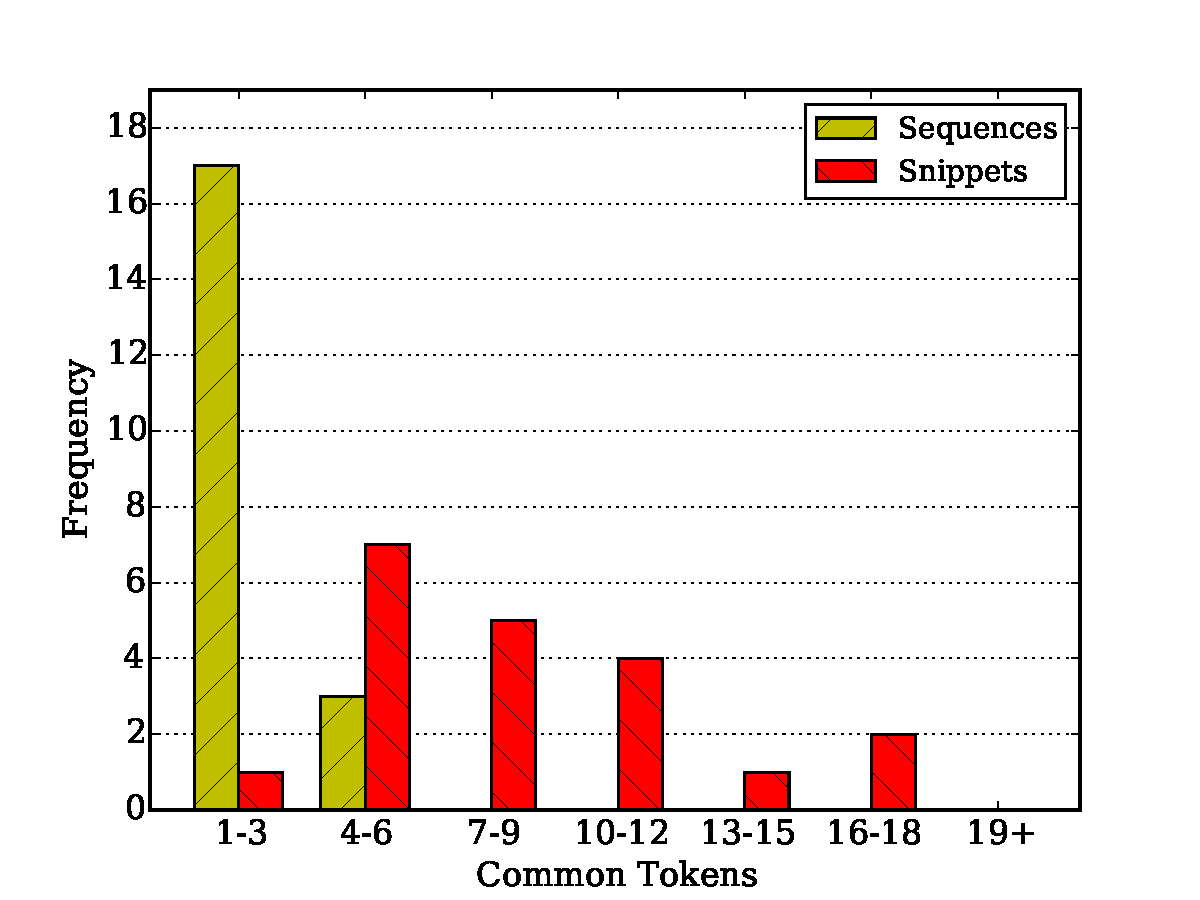
\includegraphics[width=0.45\textwidth]{results/exp5-common-tokens.pdf}}
  \end{subfloatrow}}
  {\caption[Illustration of the additional information revealed when mining snippets instead of sequences]{Figures illustrating (\subref{res:exp5-additional-info}) the additional information -in terms of Java tokens- revealed when mining snippets instead of sequences, for the top $20$ mined snippets of the $KeepUniqHDBSCANSum$ version of the system, and (\subref{res:exp5-common-tokens}) the distribution of common tokens between the mined snippets and their associated examples, when presenting snippets and sequences.}
\label{res:exp5-addit-tokens}}
\end{figure}